\documentclass[a4paper]{article}

\usepackage{graphicx}
\usepackage{html}
\usepackage{ifpdf}
\usepackage{ifthen}
\newcommand{\oofem}{\htmladdnormallink{OOFEM}{http://www.oofem.org}\ }
\newcommand{\bp}{\htmladdnormallink{Bo\v{r}ek Patz\'{a}k}{http://mech.fsv.cvut.cz/~bp/bp.html}}
\usepackage{amsmath}


\renewcommand{\topfraction}{1.99}	% 99% of page top can be a float
\renewcommand{\bottomfraction}{0.99}	% 99% of page bottom can be a float
\renewcommand{\textfraction}{0.01}	% only 1% of page must to be the text
\renewcommand{\floatpagefraction}{0.99} % 99% of whole page can be a float
\setcounter{totalnumber}{5} %maximum floating objects on one page

\newcommand{\mbf}[1]{\mbox{\boldmath$#1$}}
\newcommand{\grad}{\nabla}
\newcommand{\vect}[1]{\mathbf{#1}} % not for Greek letters
\newcommand{\tens}[1]{\pmb{#1}} % A second-order tensor

\newcommand{\strain}{\varepsilon}
\newcommand{\stress}{\sigma}
%% Definitions for PostScript output
%\newcommand{\param}[1]{mbox{\texttt{#1}}}
%\newcommand{\fieldVal}[2]{${\mbox{\#\rm\it #1}}_{\rm #2}$}
%\newcommand{\keywordnotype}[1]{\mbox{{\texttt{\textbf{#1}}}}}
%\newcommand{\keyword}[2]{$\keywordnotype{#1}_{\rm #2}$}
%\newcommand{\entKeyword}[1]{\mbox{{*\texttt{\textbf{#1}}}}}
%\newcommand{\entKeywordWithVal}[2]{*\keyword{#1}{#2}}
%\newcommand{\entKeywordInst}[1]{\mbox{{\texttt{\textit{#1}}}}}
%\newcommand{\field}[2]{\keyword{#1}{#2}~\#}
%\newcommand{\optField}[2]{[\field{#1}{#2}]}
%% Definitions for www output (using latex2html)
\newcommand{\param}[1]{{\em #1}}
\newcommand{\fieldVal}[2]{\mbox{({\it\bf{#1}\#)\tiny (#2)}}}
\newcommand{\keywordnotype}[1]{\mbox{{\it{\bf{#1}}}}}
\newcommand{\keyword}[2]{\mbox{{\keywordnotype{#1}\tiny (#2)}}}
\newcommand{\entKeyword}[1]{\mbox{{*{\bf{#1}}}}}
\newcommand{\entKeywordWithVal}[2]{\mbox{*\keyword{#1}{#2}}}
\newcommand{\entKeywordInst}[1]{\mbox{{\bf{{#1}}}}}
\newcommand{\field}[2]{\mbox{\keyword{#1}{#2}~\#}}
\newcommand{\optField}[2]{\mbox{[\field{#1}{#2}]}}
%% macros for items related to parallel
%%\newcommand{\Pmode}[1]{\begin{minipage}[t]{11cm}\textsf{#1}\end{minipage}}
\newcommand{\Pmode}[1]{{\sffamily #1}}
\newcommand{\Pparam}[1]{\param{#1}}
\newcommand{\PfieldVal}[2]{\mbox{$\langle$({\it\bf{#1}\#)\tiny (#2)}$\rangle$}}
\newcommand{\Pkeywordnotype}[1]{\mbox{$\langle${\it{\bf{#1}}}}$\rangle$}
\newcommand{\Pkeyword}[2]{\mbox{$\langle${\keywordnotype{#1}\tiny (#2)}$\rangle$}}
\newcommand{\PentKeyword}[1]{\mbox{{$\langle$*{\bf{#1}}$\rangle$}}}
\newcommand{\PentKeywordWithVal}[2]{\mbox{*\Pkeyword{#1}{#2}}}
\newcommand{\PentKeywordInst}[1]{\mbox{$\langle${\bf{{#1}}}$\rangle$}}
\newcommand{\Pfield}[2]{\mbox{$\langle$\keyword{#1}{#2}~\#$\rangle$}}
\newcommand{\PoptField}[2]{\mbox{$\langle$[\field{#1}{#2}]$\rangle$}}
\begin{htmlonly}
\newenvironment{record}[1][]{\begin{tabular}{|ll}}{\end{tabular}\\}
\newcommand{\recentry}[2]{{#1}&{#2}\\}
\end{htmlonly}
%begin{latexonly}
\newcounter{rcc}
\newenvironment{record}[1][\textwidth]{\setcounter{rcc}{0}\begin{tabular*}{#1}{|ll@{\extracolsep{\fill}}r}}{\end{tabular*}\\}
%\newenvironment{record}{\begin{tabular}{|llr}}{\end{tabular*}\\}
\newcommand{\recentry}[2]{\ifthenelse{\value{rcc}>0}{&$\backslash$ \\}{\setcounter{rcc}{1}}{#1}&{#2}}
%end{latexonly}


\begin{document}
%begin{latexonly}
\title{
\ifpdf
\oofemlnk{\centerline{
\includegraphics[width=0.7\textwidth]{oofem-logo-contour.pdf}}}
\else
\oofemlnk{\centerline{
\includegraphics[width=0.7\textwidth]{oofem-logo-contour.eps}}}
\fi
Input Data Format Specification}
\author{\bp \\ \\
Czech Technical University\\
Faculty of Civil Engineering\\
Department of Structural Mechanics\\
Th\'akurova 7, 166 29 Prague, Czech Republic
}
\maketitle
%end{latexonly}
\begin{htmlonly}
\begin{center}
  \oofemlnk{\centerline{
\includegraphics[width=0.7\textwidth]{oofem-logo-contour.eps}}}
{\Large Input Data Format Specification} \\ \\
{\bp \\
Czech Technical University\\
Faculty of Civil Engineering\\
Department of Structural Mechanics\\
Th\'akurova 7, 166 29 Prague, Czech Republic
}
\end{htmlonly}

\newpage
\tableofcontents
\newpage
\section{Introduction}
This report describes in details the format and structure of OOFEM
text input file. Input file can be created by any available text editor or can be generated
by some conversion program or by some FEM pre-processor.

\Pmode{Some parts of this document are related parallel version of the code (POOFEM). These parts are distinguished by typing the text in sans serif font family.}
\Pmode{In a parallel mode a set of input files must be provided, each one for
particular process and related partition. The input file corresponding to some
partition is called partition input file. Its name is composed from two parts. The fist part (referred as base
name) is user-defined. The second part (called partition name), divided from first part by
full-stop, is particular partition rank number. The partitions are numbered
from zero. It is assumed, that all partitions input files have the
same base name. The partition name is appended automatically to input
file name, user provides only base name on input. On the other hand,
the partition name is not appended to output file name, as specified
in output file record (see section \ref{_OutputFileRecord}).

The parallel version requires the unique global numbering  for
dof managers (nodes) and elements. The global
numbering is necessary to link partitions together. However, the dof
managers and optionally elements at interpartion boundaries,
should be explicitly  marked, in order to distinguish different type
of relations between their remote counterparts (see further).}

\section{Running the code}
\label{_running_the_code}
The program may be executed by typing\\
\texttt{oofem [option [parameter]] ...}\\
on the command line prompt with the following command line options:
\begin{itemize}
\item
{\bf -f string}\\ oofem input file name, if not present, program interactively
reads this parameter.
\item
{\bf -r int}\\
Restarts the analysis from given solution step. The corresponding
context file (*.osf) must exist.
\item
{\bf -rn}\\
Turns on the profile renumbering. Default is off. It will not work in parallel mode.
\item
{\bf -ar int}\\
Restarts the adaptive computation from given solution step.
Requires the corresponding context file (*.osf) and domain input file
(*.din) to exists. The domain input file describes the new mesh, its
syntax is identical to syntax of input file, but it does not contains
the output file record, job description record and analysis record.
\item
{\bf -qo string}\\
Redirect the standard output stream (stdout) to given file.
\item
{\bf -qe string}\\
Redirect standard error stream (stderr) to given file.
\item
{\bf -context}\\
Forces the creation of context file for each solution step.
\end{itemize}

\Pmode{
The parallel version uses the MPI (Message Passing Interface) standard for message-passing communication. Thus, to execute POOFEM program,
users must know the procedure for beginning MPI jobs on their selected computer system(s).
For instance, when using the MPICH implementation of MPI and many others, the following command initiates a program that uses eight processors: \\[2mm]
\texttt{mpirun -np 8 poofem program\_options}
}




\section{Syntax and general rules}

Input file is created by records. In the current implementation, the
particular record is represented by one line in input file.
The order of records in file is
compulsory, and is following
\begin{enumerate}
\item output file record, see section \ref{_OutputFileRecord},
\item job description record, see section \ref{_JobDescriptionRecord},
\item analysis record, see section \ref{_AnalysisRecord},
\item domain record, see section \ref{_DomainRecord},
\item output manager record, see section \ref{_OutputManagerRecord},
\item components size record, see section \ref{_ComponentsSizeRecord},
\item node \& element-side  record(s), see section \ref{_NodeElementSideRecords},
\item element record(s), see section \ref{_ElementsRecords},
\item cross section record(s), see section \ref{_CrossSectionRecords},
\item material type  record(s), see section \ref{_MaterialTypeRecords},
\item nonlocal barriers record(s), see section \ref{_NonlocalBarrierRecords},
\item load, boundary  conditions record(s), see section
  \ref{_LoadBoundaryInitialConditions},
\item initial conditions record(s), see section \ref{_InitialConditions},
\item time functions record(s), see section \ref{_TimeFunctionsRecords}.
\item optional xfem manager and associated record(s), see section \ref{_XFEMManagerRecords}
\end{enumerate}
When line begins with '\#' character, then it is skipped by parser and
provide a way, how to include comments inside input file.

Records contain many fields, each field is characterized by
keyword and its associated  field value. Some keywords have no field  values.
Except the first field, the order of remaining fields in record is
optional. There are several
exceptions, which will be described in particular sections.
The type of field value is specific to  keyword.
General format of field, characterized by keyword ``Keyword'' with
corresponding value (marked as \#) of type ``type'' is
\field{Keyword}{type}.
If keyword is variable, depending on entity type which is
described by particular record, then the keyword is preceded by star. We call such keyword
as entity keyword (For example keyword, which  describes  element
type). The possible
substitutions for entity keyword are typed using
\entKeywordInst{Typewriter} font family.
Often, many fields are specific to particular entity keyword. Then we describe
general format of record without these specific fields and we describe
them in entity keyword specific part of record description.
Sometimes, there are fields without keywords. These are usually
compulsory, with fixed position in record. Their occurrence is
described using so called named values. The format of named value is
``\fieldVal{name}{type}'', where a value of required type should be
substituted.

In a special case of analysis record, the input record can be followed
by optional meta-step input records (see section
\ref{_AnalysisRecord}). Then certain fields originally in analysis
record should appear in meta-step record instead. This is marked by
adding ``M'' superscript to keyword. Then the field format is \field{Keyword$^M$}{type}.

As already mentioned, each field value is typed. The possible types are:
\begin{itemize}
\item in - integer number.
\item rn - real number.
\item ch - character (usually for unknowns description ('d' for
displacement unknown, 't' for temperature unknown, ...).
\item ia - integer array, format of integer array is
``size~val(1)~...~val(size)'', where size, val(1),...,val(size) are
integer numbers. Values are separated by one or more spaces.
\item ra - real array, format of real array is
``size~val(1)~...~val(size)'', where size is integer number and val(1),
..., val(size) are real numbers. Values are separated by one or more spaces;
\item rm - real matrix, format of real matrix is\\
``rows~columns~\{val(1,1)~val(1,2)~...;~val(2,1)~...\}'', where ``rows'' and ``columns'' are integer numbers and val(1,1),
..., are real numbers. Columns are seperated by space or comma and lines by semicolon.
\item dc - dictionary. Dictionary consist of pairs, each pair has key
(character type) and its associated value (integer type).
Format of dictionary is
``size~key(1)~val(1)~...~key(size)~val(size)'', where size is integer
number, key(1),...,key(size) are single character values, and val(1),
..., val(size) are real numbers. Values are separated by one or more spaces;
\item rl - range list. Range list syntax is \{ number1 .. numberN (start1
end1) (start2 end2)\}. The enclosing brackets are compulsory. The range
list represent list of integer values. Single values can be specified
using single values (number1, .., NumberN). The range of values
(all numbers from startI to endI including startI and endI can be
specified using range value in the form (startI endI). The range is
described using its start and end values enclosed in parenthesis.
Any number of ranges and single values can be used to specify range list.
\item et - entity type. For  example, it describes the finite element
type. Possible type values are mentioned in specific sections.
\item s - character string. The string have to be enclosed
in quotes ("") following after corresponding keyword.
\item expr - function expression. The expression have to be enclosed
in quotes (""). The expression is evaluated by internal parser and
represent mathematical expressions as a function of certain variables.
The variable names and meaning are described in specific sections.
The usual arithmetic operators like -,+,*,/ are supported and their
evaluation order is taken into account. The evaluation order can be
changed using parenthesis. Several built-in functions are supported
(sqrt, sin, cos, tan, atan, asin and acos) - these must be typed using
lowercase letters and their arguments must be enclosed in parenthesis.
\end{itemize}

The general format of record is \\

\noindent
\begin{record}
  \recentry{}{\field{keyword1}{type} \optField{keyword2}{type}}
  \recentry{}{...} \recentry{}{\optField{keywordXX}{type}}
\end{record}

The keywords and their values are separated by one or more spaces. Please note, that a single record cooresponds to one input line in input file. \Pmode{If any keyword or field value is enclosed within angle brackets $\langle$~$\rangle$ then it is related to parallel version of oofem is not available in sequential version.
When some field is enclosed in brackets [~], then it's use is optional
and often overwrites the default behavior or adds additional (but
optional) information or property (for example adds a loading to
node). }

\section{Output file record}
\label{_OutputFileRecord}
This record has no keywords and contains character string, which
describes the path to output file. If file with the same name exists,
it will be overwritten.

\section{Job description record}
\label{_JobDescriptionRecord}
This record has no keywords and contains character string, which
describes the job. This description will appear in the output
file.

\section{Analysis record}
\label{_AnalysisRecord}
This record describes the type of analysis, which should be
performed. The general format of this record can be specified in
\begin{itemize}
\item ``standard-syntax''\\
  \begin{record}[0.9\textwidth]
    \recentry{\entKeyword{AnalysisType}}{\field{nsteps}{in}} \recentry{}{\optField{renumber}{in}}
    \recentry{}{\field{attributes}{string}} \recentry{}{\optField{ninitmodules}{in}} \recentry{}{\optField{nmodules}{in}} \recentry{}{\optField{nxfemman}{in}}
  \end{record}
\item ``meta step-syntax''\\
  \begin{record}[0.9\textwidth]
    \recentry{\entKeyword{AnalysisType}}{\field{nmsteps}{in}}
    \recentry{}{\optField{ninitmodules}{in}} \recentry{}{\optField{nmodules}{in}} \recentry{}{\optField{nxfemman}{in}}
  \end{record}
  immediately followed by \param{nmsteps} meta step records with the following syntax:\\
  \begin{record}[0.9\textwidth]
    \recentry{}{\field{nsteps}{in} \field{attributes}{string}}
  \end{record}
  The \param{nmsteps} parameter determines the number of ``metasteps''. The
meta step represent sequence of solution steps with common attributes.
There is expected to be \param{nmsteps} subsequent metastep records.
The meaning of meta step record parameters (or analysis record
parameters in ``standard syntax'') is following:
\begin{itemize}
\item \param{nsteps} - determines number of subsequent solution steps
within me\-ta\-step.
Nonzero value of optional parameter \param{renumber} turns on the
equation renumbering to optimize the profile of characteristic matrix
(uses Sloan algorithm). By default, profile optimization is not
performed. It will not work in parallel mode.
\item \param{attributes} - contains the metastep related attributes of
analysis (and solver), which are valid for corresponding solution
steps within meta step. If used in standard syntax, the attributes are
valid for all solution step.
\item \param{ninitmodules} - number of initialization module records for given
problem. The initialization modules are specified after meta step section (or
after analysis record, if no metasteps are present). Initialization modules
allow to initialize the state variables by values previously computed by 
external software. The available initialization modules are described in section
\ref{InitModulesSec}.
\item \param{nmodules} - number of export module records for given
problem. The export modules are specified after initialization modules. Export modules
allow to export computed data into external software for
postprocessing. The available export modules are described in section
\ref{ExportModulesSec}.
\item \param{nxfemman} - number of xfem managers. Xfem managers wrap eXtended Finite Element (xfem) data: they  manage the list of enrichment items and associated enrichment functions, and their geometry representation. The number of xfem managers required is problem dependent, typically a single xfem manager is used. The syntax of xfem manager record and related records is described in section \ref{_XFEMManagerRecords}.
\end{itemize}

\end{itemize}
Not all of analysis types support the metastep syntax, and if
not mentioned, the standard-syntax is expected.
Currently, supported analysis types are

\begin{itemize}
\item Linear static analysis, see section \ref{LinearStatic},
\item Eigen value dynamic, see section \ref{EigenValueDynamic},
\item Direct explicit  nonlinear dynamics, see section
\ref{NlDEIDynamic},
\item Direct explicit (linear) dynamics, see section \ref{DEIDynamic},
\item Implicit linear dynamic, see section \ref{DIIDynamic},
\item Incremental {\bf linear} static problem, see section \ref{IncrementalLinearStatic},
\item Non-linear static analysis, see section \ref{NonLinearStatic}.
\end{itemize}

\subsection{Linear static analysis}
\label{LinearStatic}
\begin{record}
\recentry{\entKeywordInst{LinearStatic}}{\field{nsteps}{in}}
\recentry{}{\optField{renumber}{in}}
\recentry{}{\optField{sparselinsolverparams}{}}
\recentry{}{\optField{sparselinsolverparams}{}}
\end{record}

Linear static analysis.
Parameter \param{nsteps} indicates the number of loading cases.
Series of loading cases is maintained as sequence of time-steps.
For each load case an auxiliary time-step is generated with time
equal to load case number.
Load vectors for each load case are formed as load vectors at
this auxiliary time.

Nonzero value of optional parameter \param{renumber} turns on the
equation renumbering to optimize the profile of characteristic matrix
(uses Sloan algorithm). By default, profile optimization is not
performed. It will not work in parallel mode.

The  \param{sparselinsolverparams} parameter describes the sparse
linear solver attributes and is explained in section \ref{sparselinsolver}.
\Pmode{Can be used in parallel mode. The input record must be the same
for all processors. At present, parallel version requires PETSc module.}


\subsection{LinearStability}
\label{LinearStability}
\begin{record}
\recentry{\entKeywordInst{LinearStability}}{\field{nroot}{in}}
\recentry{}{\optField{renumber}{in}}
\recentry{}{\field{rtolv}{rn}} \recentry{}{\optField{eigensolverparams}{}}
\end{record}
Solves linear stability problem. Only first \param{nroot} smallest
eigenvalues and corresponding eigenvectors will be computed.
Relative convergence tolerance is specified using \param{rtolv} parameter.

Nonzero value of optional parameter \param{renumber} turns on the
equation renumbering to optimize the profile of characteristic matrix
(uses Sloan algorithm). By default, profile optimization is not
performed. It will not work in parallel mode.

The \param{eigensolverparams} parameter describes the sparse
linear solver attributes and is explained in section \ref{eigensolverssection}.
\Pmode{Can be used in parallel mode. The input record must be the same
for all processors. Parallel version requires PETSc and SLEPc modules.}

\subsection{EigenValueDynamic}
\label{EigenValueDynamic}
\begin{record}
\recentry{\entKeywordInst{EigenValueDynamic}}{\field{nroot}{in}}
\recentry{}{\optField{renumber}{in}}
\recentry{}{\field{rtolv}{rn}} \recentry{}{\optField{eigensolverparams}{}}
\end{record}

Represents the eigen value dynamic analysis.
Only \param{nroot} smallest eigenvalues and corresponding
eigenvectors will be computed. Relative convergence criteria is
governed using \param{rtolv} parameter.
Nonzero value of optional parameter \param{renumber} turns on the
equation renumbering to optimize the profile of characteristic matrix
(uses Sloan algorithm). By default, profile optimization is not
performed. It will not work in parallel mode.

The \param{eigensolverparams} parameter describes the sparse
linear solver attributes and is explained in section \ref{eigensolverssection}.
\Pmode{Can be used in parallel mode. The input record must be the same
for all processors. Parallel version requires PETSc and SLEPc modules.}


\subsection{NlDEIDynamic}
\label{NlDEIDynamic}
\begin{record}
\recentry{\entKeywordInst{NlDEIDynamic}}{\field{nsteps}{in}}
\recentry{}{\optField{renumber}{in}}
\recentry{}{\field{dumpcoef}{rn}} \recentry{}{\optField{deltaT}{rn}}
\end{record}

Represents the direct explicit  nonlinear dynamic  integration.
The central difference method with diagonal mass matrix is used,
damping matrix is assumed to be proportional to mass matrix, $\mbf{C}
= {\rm dumpcoef} * \mbf{M}$, where
$\mbf{M}$ is diagonal mass matrix. \param{deltaT} is time step length used for
integration, which may be reduced by program in order to satisfy
solution stability conditions. Parameter \param{nsteps} specifies
how many time steps will be analyzed.
Nonzero value of optional parameter \param{renumber} turns on the
equation renumbering to optimize the profile of characteristic matrix
(uses Sloan algorithm). By default, profile optimization is not
performed. It will not work in parallel mode.
\\ \\
\noindent
\begin{record}
\recentry{\PentKeywordInst{PNlDEIDynamic}}{\Pfield{nsteps}{in}}
\recentry{}{\Pfield{dumpcoef}{rn}} \recentry{}{\PoptField{deltaT}{rn}}
\recentry{}{\PentKeyword{commode}} \recentry{}{\PoptField{nonlocalext}{}}
\end{record}

\Pmode{
Represents the parallel direct explicit  nonlinear dynamic  integration.
The central difference method with diagonal mass matrix is used,
damping matrix is assumed to be proportional to mass matrix, $\mbf{C}
= {\rm dumpcoef} * \mbf{M}$, where
$\mbf{M}$ is diagonal mass matrix. \param{deltaT} is time step length used for
integration, which may be reduced by program in order to satisfy
solution stability conditions. Parameter \param{nsteps} specifies
how many time steps will be analyzed.
The \PentKeyword{commode} keyword can be one from following:
\begin{itemize}
\item \entKeywordInst{nodecutmode} - indicates the node cut partitioning scheme is
used. The cut is led along element edges or surfaces (see
figures \ref{nodecut}, \ref{nodecut-lm}, and \ref{nodecut-nlm}).
\item \entKeywordInst{elementcutmode} - the element cut partitioning is used. The
partitioning cut led across the element edges or surfaces (see
figures \ref{elmentcut} and \ref{elmentcut-lm}).
\end{itemize}
\Pmode{
The \param{nonlocalext} turns on the nonlocal constitutive
extension. The extension considers a band of remote elements involved
in computation of nonlocal variables (see fig. \ref{nodecut-nlm} illustrating
this approach for node-cut partitioning).
}
}

\subsection{DEIDynamic}
\label{DEIDynamic}

\begin{record}
\recentry{\entKeywordInst{DEIDynamic}}{\field{nsteps}{in}}
\recentry{}{\field{dumpcoef}{rn}} \recentry{}{\optField{deltaT}{rn}}
\end{record}

Represent the {\bf linear} explicit
integration scheme for dynamic problem solution. The central difference method with diagonal mass matrix is used,
damping matrix is assumed to be proportional to mass matrix, $\mbf{C} = {\rm dumpcoef} * \mbf{M}$, where
$\mbf{M}$ is diagonal mass matrix. \param{deltaT} is time step length used for
integration, which may be reduced by program in order to satisfy
solution stability conditions. Parameter \param{nsteps} specifies
how many time steps will be analyzed.

\subsection{DIIDynamic}
\label{DIIDynamic}

\begin{record}
\recentry{\entKeywordInst{DIIDynamic}}{\field{nsteps}{in}}
\recentry{}{\optField{renumber}{in}}
\recentry{}{\field{deltaT}{rn}} \recentry{}{\field{alpha}{rn}} \recentry{}{\field{beta}{rn}}
\recentry{}{\field{Psi}{rn}}
\end{record}

Represents direct implicit integration of linear dynamic
problems. Damping is modeled as Rayleigh damping $(\mbf{c} =
\rm{alpha}*\mbf{M} + \rm{beta} * \mbf{K})$. Parameter \param{Psi} determines
integration method used, for\param{Psi} = 1 the Newmark and for \param{Psi} $\ge$ 1.37 the Wilson method
will be used. Parameter \param{deltaT} is required time integration
step length.
Nonzero value of optional parameter \param{renumber} turns on the
equation renumbering to optimize the profile of characteristic matrix
(uses Sloan algorithm). By default, profile optimization is not
performed. It will not work in parallel mode.

\subsection{IncrementalLinearStatic}
\label{IncrementalLinearStatic}

\begin{record}
\recentry{\entKeywordInst{IncrLinearStatic}}{\field{endOfTimeOfInterest}{rn}}
\recentry{}{\field{pre\-scri\-bed\-Ti\-mes}{ra}}
\recentry{}{\optField{renumber}{in}}
\end{record}


Represents incremental {\bf linear} static problem.
The problem is solved as series of linear solutions and is intended to
be used for solving linear creep problems or incremental perfect plasticity.
Nonzero value of optional parameter \param{renumber} turns on the
equation renumbering to optimize the profile of characteristic matrix
(uses Sloan algorithm). By default, profile optimization is not
performed. It will not work in parallel mode.

Supports the changes of static scheme (applying, removing and changing  boundary conditions)
during the analysis.

Response is computed in times defined by \param{pre\-scri\-bed\-Ti\-mes}
array. These times should include times, when generally the  boundary
conditions are changing, and in other times of interest. (For linear creep
analysis, the values should be uniformly distributed on log-time scale, if no change in
loading or boundary conditions). The time at the end of interested is
specified using \param{endOfTimeOfInterest} parameter.

\subsection{NonLinearStatic}
\label{NonLinearStatic}
\entKeywordInst{NonLinearStatic} \\
Non-linear static analysis. The problem can be solved under
direct load or displacement control, indirect control, or by
their arbitrary combination.
\Pmode{Can be used in parallel mode. The input record must be the same
for all processors. At present, parallel version requires PETSc module.}
By default all
material nonlinearities will be included, geometrical not.
To include geometrically nonlinear effect one must specify
level of non-linearity in element records.
There are two different ways, how to specify the parameters - the
extended and standard syntax.
\subsubsection{Extended syntax}
The extended syntax uses the ``metastep'' concept and has the
following format:
%%\begin{enumerate}
%%\item[0]

\noindent
\begin{record}
\recentry{\entKeywordInst{NonLinearStatic}}{\optField{nmsteps}{in}}
\recentry{}{\field{nsteps}{in}}
\recentry{}{\optField{renumber}{in}}
\recentry{}{\optField{contextOutputStep}{in}}
\recentry{}{\optField{sparselinsolverparams}{string}}
\recentry{}{\optField{nonlinform}{in}}
\recentry{}{\PoptField{nonlocstiff}{in}} \recentry{}{\PoptField{nonlocalext}{}} \recentry{}{\PoptField{loadbalancing}{}}
\end{record}
This record is immediately followed by metastep records with the format described bellow.
The analysis parameters have following meaning
\begin{itemize}
\item \param{nmsteps} - determines the number of
``metasteps'', default is 1.
\item \param{nsteps} - determines number of solution steps.
\item Nonzero value of optional parameter \param{renumber} turns on the
equation renumbering to optimize the profile of characteristic matrix
(uses Sloan algorithm). By default, profile optimization is not
performed. It will not work in parallel mode.
\item \param{contextOutputStep} - causes the context file to be
created for every con\-text\-Out\-put\-Step-th step and when needed. Useful for
postprocessing.
\item The  \param{sparselinsolverparams} parameter describes the sparse
linear solver attributes and is explained in section \ref{sparselinsolver}.
\item \param{nonlinform} - formulation of non-linear problem. If == 1 (default), total Lagrangian formulation in undeformed original shape is used (first-order theory). If == 2, the equlibrated displacements are added to original ones and updated in each time step (second-order theory).
\item \Pmode{\param{nonlocstiff} - determines whether the tangent stiffness
extension for nonlocal models is activated. If == 0 (default) this
option is not active. If == 1 the support for nonlocal tangent
stiffness is activated.}
\item \Pmode{The \param{nonlocalext} turns on the nonlocal constitutive
extension. The extension considers a band of remote elements involved
in computation of nonlocal variables (see fig. \ref{nodecut-nlm} illustrating
this approach for node-cut partitioning)}.
\item \Pmode{The  \param{loadbalancing} parameter describes the dynamic load balancing
attributes and is explained in section \ref{dynamicloadbalancing}}.
\end{itemize}

%The metasteps \fieldVal{num}{in} is the metastep number and the
%\param{nsteps} - determines number of solution steps for corresponding
%metastep.
\noindent
The metastep record has following general syntax:\\
\begin{record}
\recentry{\hspace{10mm}}{\field{nsteps}{in}}
\recentry{}{\optField{controllmode}{in}}
\recentry{}{\optField{deltat}{rn}} \recentry{}{\optField{stiffmode}{in}}
\recentry{}{\optField{refloadmode}{in}} \recentry{}{\field{solverParams}{}}
\recentry{}{\optField{sparselinsolverparams}{string}} \recentry{}{\optField{donotfixload}{}}
\end{record}

where
\begin{itemize}
\item[-] \param{controllmode} - determines the type of solution
control used for corresponding meta step. if == 0 then indirect
control will be used to control solution process (arc-length method, default). if == 1
then direct displacement or load control will be used (Newton-Raphson solver). In the later
mode, one can apply the prescribed load increments as well as
control displacements.
\item[-] \param{deltaT} - is time step length. If not specified, it is
set equal to 1,0. Each solution step has associated the corresponding
intrinsic time, at which the loading is generated. The \param{deltaT}
determines the spacing between solution steps on time scale.
\item[-] \param{stiffMode} - If == 0 (default) then tangent stiffness will be used
at new step beginning and whenever numerical method will ask for
stiffness update. If == 1 the use of secant tangent will be forced.
The secant stiffness will be used at new step beginning
and whenever numerical method will ask for stiffness update.
If == 2 then original elastic stiffness will
be used during the whole solution process.
\item[-] The \param{refloadmode} parameter determines how the reference force load vector
is obtained from given totalLoadVector and initialLoadVector.
The initialLoadVector describes the part of loading which does not scale. Works only for force loading, other non-force components (temperature, prescribed displacements should always given in total values).
If refLoadInputMode is 0 (rlm\_total, default) then the reference incremental load vector is defined as
totalLoadVector assembled at given time.
If refLoadInputMode is 1 (rlm\_inceremental) then the reference load vector is
obtained as incremental load vector at given time.
\item[-] \param{solverParams} - parameters of solver. The solver type
is determined using \param{controllmode}.
\item The  \param{sparselinsolverparams} parameter describes the sparse
linear solver attributes and is explained in section
\ref{sparselinsolver}.
\item[-] By default, reached load at the end of
metastep will be maintained in subsequent steps as fixed, non scaling
load and load level will be reset to zero. This can be changed using keyword \param{donotfixload}, which if
present, causes the loading to continue, not resetting the load
level. For the indirect control the reached loading will not be
fixed, however, the new reference loading vector will be assembled for
the new metastep.
\end{itemize}

The direct solver corresponds to \param{controllmode}=1 and the Newton-Raphson solver is used.
Under the direct control, the total load
vector assembled for specific solution step represents the load level,
where equilibrium is searched. The implementation supports also
displacement control -  it is possible to prescribe one or more
displacements by applying ``quasi prescribed'' boundary
condition(s)\footnote{Hovewer, the problem does not supports the
changes of static system. But it is possible to apply direct
displacement control without requiring BC applied (see nrsolver
documentation). Therefore it is possible to combine
direct displacement control with direct load control or indirect
control.}
The load level then represents the
time, where the equilibrium has been found. The Newton-Raphson solver parameters (\param{solverParams}) for
load-control are:\\
\begin{record}
\recentry{\hspace{10mm}}{\field{maxiter}{in}}
\recentry{}{\optField{minsteplength}{in}}
\recentry{}{\optField{minIter}{in}}
\recentry{}{\optField{manrmsteps}{in}}
\recentry{}{\optField{ddm}{ia} \optField{ddv}{ra} \optField{ddltf}{in}}
\recentry{}{\optField{linesearch}{in} \optField{lsearchamp}{rn}}
\recentry{}{\optField{lsearchmaxeta}{rn} \optField{lsearchtol}{rn}}
\recentry{}{[\field{nccdg}{in} \field{ccdg1}{ia} ... \field{ccdgN}{ia}  ]}
\recentry{}{\field{rtolv}{} [\field{rtolf}{} \field{rtold}{} ]}
\end{record}
where
\begin{itemize}
\item \param{maxiter} determines the maximum
number of iterations allowed to reach equilibrium. If equilibrium is
not reached, the step length (corresponding to time) is reduced.
\item \param{minsteplength} parameter is the minimum step length
allowed.
\item \param{minIter} - minimum number of iterations which always proceed during the iterative solution.
\item If \param{manrmsteps} parameter is nonzero, then the modified
N-R scheme is used, with the stiffness updated after
\param{manrmsteps} steps.
\item \param{ddm} is array specifying the degrees of freedom,
which displacements are controlled.
Let the number of these DOFs is N.
The format of \param{ddm} array is 2*N dofman1 idof1
dofman2 idof2 ... dofmanN idofN, where the dofmani is the number of i-th dof manager  and idofi is the
corresponding DOF number.
\item \param{ddv} is array of relative weights of controlled
displacements, the size should be equal to N. The actual value of
prescribed dofs is defined as a product of its weight and the value of
load time function specified using \param{ddltf} parameter (see
below).
\item \param{ddltf} number of load time function, which is used to
evaluate the actual displacements of controlled dofs.
\item \param {linesearch} nonzero value turns on line search
  algorithm. The \param{lsearchtol} defines tolerance (default value
  is 0.8), amplification
  factor can be specified using \param{lsearchamp} parameter (should
  be in interval $(1,10)$), and parameter \param{lsearchmaxeta}
  defines maximum limit on the length of iterative step (allowed range
  is $(1.5,15)$).
\item \param{nccdg} allows to define one or more DOF groups, that are used for evaluation of convergence criteria. Each DOF is checked if it is a member of particular group and in this case its contribution is taken into account when evaluating the convergence criteria for that group. By default, if \param{nccdg} is not specified, one group containing all DOF types is created. The value of \param{nccdg} parameter defines the number of DOF type groups. For each group, the corresponding DOF types need to be specified using \param{ccdg\#} parameter, where '\#' should be replaced by group number (numbering starts from 1). This array contains the DofIDItem values, that identify the physical meaning of DOFs in the group. The values and their physical meaning is defined by DofIDItem enum type (see src/oofemlib/dofiditem.h for reference).
\item \param{rtolv} determines relative convergence norm (both for displacement
iterative change vector and for residual unbalanced force vector). Optionally, the \param{rtolf} and \param{rtold} parameters can be used to define
independent relative convergence crteria for unbalanced forces and displacement
iterative change. If the default convergence criteria is used,
the parameters \param{rtolv},\param{rtolf}, and \param{rtold} are real values. If the convergence criteria DOF groups are used (see bellow the description of \param{nccdg} parameter) then they should be specified as real valued arrays of \param{nccdg} size, and individual values define relative convergence criteria for each individual dof group.
\end{itemize}

The indirect solver corresponds to \param{controllmode}=0 and the CALM
solver is used. The value of reference load vector is determined by
\param{refloadmode} parameter mentioned above at the first step of
each metastep. {\em However, the user must ensure, that the same value of
reference load vector could be obtained for all solution steps of
particular metastep (this is necessary for restart and adaptivity to work)}.
The corresponding meta step solver parameters (\param{solverParams}) are:\\
\begin{record}
\recentry{\hspace{10mm}}{\field{Psi}{rn}}
\recentry{}{\field{MaxIter}{in}}
\recentry{}{\field{stepLength}{rn}}
\recentry{}{\optField{min\-Step\-Le\-ngth}{in}}
\recentry{}{\optField{initialStepLength}{rn}}
\recentry{}{\optField{forcedInitialStepLength}{rn}}
\recentry{}{\optField{reqIterations}{in}}
\recentry{}{\optField{minIter}{in}}
\recentry{}{\optField{manrmsteps}{in}}
\recentry{}{\optField{hpcmode}{in} \optField{hpc}{ia} \optField{hpcw}{ia}}
\recentry{}{\optField{linesearch}{in} \optField{lsearchamp}{rn}}
\recentry{}{\optField{lsearchmaxeta}{rn} \optField{lsearchtol}{rn}}
\recentry{}{[\field{nccdg}{in} \field{ccdg1}{ia} ... \field{ccdgN}{ia}]}
\recentry{}{\field{rtolv}{} [\field{rtolf}{} \field{rtold}{} ]}
\end{record}
where
\begin{itemize}
\item \param{Psi} - CALM $\Psi$ control parameter. For $\Psi$ = 0
displacement control is applied. For nonzero values the load control
applies together with displacement control (ALM). For large $\Psi$
load control apply.
\item \param{MaxIter} - determines the maximum number of iteration allowed to
reach equilibrium state. If this limit is reached, restart follows
with smaller step length.
\item \param{stepLength} - determines the maximum value of arc-length (step length).
\item \param{min\-Step\-Le\-ngth} - minimum step length. The step length will never be
smaller. If convergence problems are encountered and step length cannot
be decreased, computation terminates.
\item \param{initialsteplength} - determines the initial step length (the arc-length). If not provided, the maximum step length (determined by \param{stepLength} parameter) will be used as the value of initial step length. 
\item \param{forcedInitialStepLength} - When simulation is restarted, the last predicted step length is used. Use \param{forcedInitialStepLength} parameter to override the value of step length. This parameter will also override the value of initial step length set by \param{initialsteplength} parameter.
\item \param{reqIterations} - approximate number of iterations controlled by changing the step length.
\item \param{minIter} - minimum number of iterations which always proceed during the iterative solution. \param{reqIterations} are set to be the same, \param{MaxIter} are increased if lower.
\item \param{manrmsteps} - Forces the use of accelerated
Newton Raphson met\-hod, where stiffness is updated after
\param{manrmsteps} steps. By default, the modified NR
method is used (no stiffness update).
\item \param{hpcmode} Parameter determining the alm mode.
Possible values are: 0 - (default) full ALM with quadratic constrain and
all dofs, 1 - (default, if \param{hpc} parameter used) full ALM with quadratic constrain, taking into account
only selected dofs (see \param{hpc} param), 2 - linearized constrain
in displacements only, taking into account only selected dofs with
given weight (see \param{hpc} and \param{hpcw} parameters).
\item \param{hpc} - Special parameter for Hyper-plane control, when only
selected DOFS are taken account in ALM step length
condition. Important mainly for material nonlinear problems with
strong localization. This array selects the degrees of freedom,
which displacements are controlled. Let the number of these DOFs is N.
The format of \param{ddm} array is 2*N dofman1 idof1
dofman2 idof2 ... dofmanN idofN, where the dofmani is the number of i-th dof manager  and idofi is the
corresponding DOF number.
\item \param{hpcw} - Array of dof weights in linear constraint. The
dof ordering is determined by \param{hpc} param, size of array should
be N.
\item \param{linesearch} nonzero value turns on line search
  algorithm. The \param{lsearchtol} defines tolerance, amplification
  factor can be specified using \param{lsearchamp} parameter (should
  be in interval $(1,10)$), and parameter \param{lsearchmaxeta}
  defines maximum limit on the length of iterative step (allowed range
  is $(1.5,15)$).
\item \param{nccdg} allows to define one or more DOF groups, that are used for evaluation of convergence criteria. Each DOF is checked if it is a member of particular group and in this case its contribution is taken into account when evaluating the convergence criteria for that group. By default, if \param{nccdg} is not specified, one group containing all DOF types is created. The value of \param{nccdg} parameter defines the number of DOF type groups. For each group, the corresponding DOF types need to be specified using \param{ccdg\#} parameter, where '\#' should be replaced by group number (numbering starts from 1). This array contains the DofIDItem values, that identify the physical meaning of DOFs in the group. The values and their physical meaning is defined by DofIDItem enum type (see src/oofemlib/dofiditem.h for reference).
\item \param{rtolv} determines relative convergence norm (both for displacement
iterative change vector and for residual unbalanced force vector). Optionally, the \param{rtolf} and \param{rtold} parameters can be used to define
independent relative convergence crteria for unbalanced forces and displacement
iterative change. If the default convergence criteria is used,
the parameters \param{rtolv},\param{rtolf}, and \param{rtold} are real values. If the convergence criteria DOF groups are used (see bellow the description of \param{nccdg} parameter) then they should be specified as real valued arrays of \param{nccdg} size, and individual values define relative convergence criteria for each individual dof group.
\end{itemize}

\subsubsection{Standard syntax}
In this case, all parameters (for analysis as well as for the solver)
are supplied in analysis record. The default meta step is created for
all solution steps required. Then the meta step attributes are
specified within analysis record. The format of analysis record is
then following\\

\noindent
\begin{record}
\recentry{\entKeywordInst{NonLinearStatic}}{\field{nsteps}{in}}
\recentry{}{\optField{nonlocstiff}{in}}
\recentry{}{\optField{contextOutputStep}{in}} \recentry{}{\optField{controllmode}{in}}
\recentry{}{\optField{deltat}{rn}}
\recentry{}{\field{rtolv}{rn}} \recentry{}{\optField{stiffmode}{in}} \recentry{}{\field{lstype}{in}}
\recentry{}{\field{smtype}{in}} \recentry{}{\field{solverParams}{}}
\recentry{}{\optField{nonlinform}{in}}
\recentry{}{\PoptField{nonlocstiff}{in}}
\recentry{}{\PoptField{nonlocalext}{}} \recentry{}{\PoptField{loadbalancing}{}}
\end{record}
The meaning of parameters is the same as for extended syntax.

%
\subsection{Adaptive linear static}
\label{AdaptiveLinearStatic}
\begin{record}
\recentry{\entKeywordInst{Adaptlinearstatic}}{\field{nsteps}{in}}
\recentry{}{\optField{renumber}{in}}
\recentry{}{\optField{sparselinsolverparams}{}} \recentry{}{\optField{meshpackage}{in}}
\recentry{}{\field{errorestimatorparams}{}}
\end{record}
Adaptive linear static analysis. Multiple loading cases are not
supported. Due to linearity of a problem, the complete reanalysis from
the beginning is done after adaptive remeshing.
After first step the error is estimated, information about required density is generated
(using mesher interface) and solution terminates. If the error
criteria is not satisfied, then the new mesh
and corresponding input file is generated and new analysis should be
performed until the error is acceptable.
Currently, the available error estimator for linear problems is
Zienkiewicz-Zhu. Please note, that adaptive framework requires
specific functionality provided by elements and material models. For
details, see element and material model manuals.
\begin{itemize}
\item[-]
Parameter \param{nsteps} indicates the number of loading cases.
Should be set to 1.
\item[-]
Nonzero value of optional parameter \param{renumber} turns on the
equation renumbering to optimize the profile of characteristic matrix
(uses Sloan algorithm). By default, profile optimization is not
performed. It will not work in parallel mode.
\item[-]
The  \param{sparselinsolverparams} parameter describes the sparse
linear solver attributes and is explained in section \ref{sparselinsolver}.
\item[-]
The \param{meshpackage} parameter selects the mesh package interface,
which is used to generate information about required mesh density for
new remeshing. The supported interfaces are explained in section
\ref{meshpackages}. By default, the T3d interface is used.
\item[-]
The \param{errorerestimatorparams} parameter contains the parameters
of Zien\-kie\-wicz Zhu Error Estimator. These are described in section \ref{errorestimators}.
\end{itemize}

\subsection{Adaptive nonlinear static}

\begin{record}
\recentry{\entKeywordInst{Adaptnlinearstatic}}{\field{Nonlinearstaticparams}{}}
\recentry{}{\optField{equilmc}{in}} \recentry{}{\optField{renumber}{in}} \recentry{}{\optField{meshpackage}{in}}
\recentry{}{\optField{eetype}{}} \recentry{}{\field{errorestimatorparams}{}}
\end{record}

Represents Adaptive Non-LinearStatic problem. Solution is performed  as a series of increments (loading or displacement).
The error is estimated at the end of each load increment (after
equilibrium is reached), and based on reached error, the computation
continues, or the new mesh densities are generated and solution
stops. Then the new discretization should be generated.
The truly adaptive approach is supported, so the computation can be
restarted from the last step (see section \ref{_running_the_code}), solution is mapped to new mesh (separate
solution step) and new load increment is applied. Of course, one can start the analysis from
the very beginning using new mesh. Currently, the available
estimators/indicators include only linear
Zienkiewicz-Zhu estimator and scalar error indicator. Please note, that adaptive framework requires
specific functionality provided by elements and material models. For
details, see element and material model manuals.
\begin{itemize}
\item[-]
Set of parameters \param{Nonlinearstaticparams} are related to
nonlinear analysis. They are described in section
\ref{NonLinearStatic}.
\item[-]
Parameter \param{equilmc} determines, whether after mapping of primary
and internal variables to new mesh the equilibrium is restored or not
before new load increment is applied. The possible values are: 0
(default), when no equilibrium is restored, and 1 forcing the
equilibrium to be restored before applying new step.
\item[-]
The \param{meshpackage} parameter selects the mesh package interface,
which is used to generate information about required mesh density for
new remeshing. The supported interfaces are explained in section
\ref{meshpackages}. By default, the T3d interface is used.
\item[-]
Parameter \param{eetype} determines the type of error
estimator/indicator to be used. The parameters
\param{errorestimatorparams} represent set of parameters corresponding
to selected error estimator. For description, follow to section
\ref{errorestimators}.
\end{itemize}
%

\subsection{Stationary transport problem}
\label{StationaryTransport}

\begin{record}
\recentry{\entKeywordInst{StationaryProblem}}{\field{nsteps}{in}}
\recentry{}{\optField{renumber}{in}} \recentry{}{\optField{sparselinsolverparams}{}}
\recentry{}{\optField{exportfields}{}} \recentry{}{\optField{atomicfields}{in}}
\end{record}

Stationary transport problem.
Series of loading cases is maintained as sequence of time-steps.
For each load case an auxiliary time-step is generated with time
equal to load case number.
Load vectors for each load case are formed as load vectors at
this auxiliary time.
The  \param{sparselinsolverparams} parameter describes the sparse
linear solver attributes and is explained in section \ref{sparselinsolver}.
Nonzero value of optional parameter \param{renumber} turns on the
equation renumbering to optimize the profile of characteristic matrix
(uses Sloan algorithm). By default, profile optimization is not
performed. It will not work in parallel mode.

If the present problem is used within the context
of staggered-like analysis, the temperature field obtained by the
solution can be exported and made available to any subsequent
analyses. For example, temperature field obtained by present analysis
can be taken into account in subsequent mechanical analysis.
To allow this, the temperate must be ``exported''. This can be done
by adding \param{exportfields} parameter, followed by
\param{atomicfields} array. This array contains the atomic field
identifiers, which tell the problem to register its primary unknowns
under given atomic identifiers. Currently available atomic ids are:
Temperature (corresponding value is 1).
Then the subsequent analyses can get access to exported fields (via
atomic id) and take them into account, if they support such feature.

\subsection{Transient transport problem - linear case}
\label{LinearTransientTransport}

\begin{record}
\recentry{\entKeywordInst{NonStationaryProblem}}{\field{nsteps}{in}}
\recentry{}{\optField{renumber}{in}} \recentry{}{\field{deltaT}{rn}} \recentry{}{\field{alpha}{rn}}
\recentry{}{\optField{lumpedcapa}{}} \recentry{}{\optField{sparselinsolverparams}{}}
\recentry{}{\optField{exportfields}{}} \recentry{}{\optField{atomicfields}{in}}
\end{record}

{\bf Linear} implicit
integration scheme for transient transport problems. The generalized
midpoint rule (sometimes called $\alpha$-method) is used for time discretization, with alpha parameter,
which has limits $0\le\alpha\le1$. For $\alpha=0$ explicit Euler
forward method is obtained, for $\alpha=0.5$ implicit trapezoidal rule
is recovered, which is unconditionally stable, second-order accurate
in $\Delta t$, and $\alpha=1.0$ yields implicit Euler backward method,
which is unconditionally stable, and first-order accurate
in $\Delta t$. \param{deltaT} is time step length used for
integration, \param{nsteps} parameter specifies
number of time steps to be solved.
Nonzero value of optional parameter \param{renumber} turns on the
equation renumbering to optimize the profile of characteristic matrix
(uses Sloan algorithm). By default, profile optimization is not
performed. It will not work in parallel mode.
If \param{lumpedcapa} is set, then the stabilization of numerical
algorithm using lumped capacity matrix will be used, reducing the
initial oscillations.
See section \ref{sparselinsolver} for explanation of
\param{exportfields} and \param{atomicfields} parameters.
Note: This problem type {\bf requires transport module} and it
can be used only when this module is included in your oofem
configuration.

Note: This problem type {\bf requires transport module} and it
can be used only when this module is included in your oofem
configuration.

\subsection{Transient transport problem - nonlinear case}
\label{TransientTransport}

\begin{record}
\recentry{\entKeywordInst{NlTransientTransportProblem}}{\field{nsteps}{in}}
\recentry{}{\optField{renumber}{in}}
\recentry{}{\field{deltaT}{rn}} \recentry{}{\field{alpha}{rn}} \recentry{}{\optField{lumpedcapa}{}}
\recentry{}{\optField{nsmax}{in}} \recentry{}{\field{rtol}{rn}} \recentry{}{\optField{manrmsteps}{in}}
\recentry{}{\optField{sparselinsolverparams}{}}
\recentry{}{\optField{exportfields}{}} \recentry{}{\optField{atomicfields}{in}}
\end{record}

Implicit
integration scheme for transient transport problems. The generalized
midpoint rule (sometimes called $\alpha$-method) is used for time discretization, with alpha parameter,
which has limits $0\le\alpha\le1$. For $\alpha=0$ explicit Euler
forward method is obtained, for $\alpha=0.5$ implicit trapezoidal rule
is recovered, which is unconditionally stable, second-order accurate
in $\Delta t$, and $\alpha=1.0$ yields implicit Euler backward method,
which is unconditionally stable, and first-order accurate
in $\Delta t$. \param{deltaT} is time step length used for
integration, \param{nsteps} parameter specifies
number of time steps to be solved. Parameter \param{maxiter} determines the maximum
number of iterations allowed to reach equilibrium (default is 30).
The convergence is reached, when norms of both residual fluxes and iterative
change of solution vector is less than the value given by \param{rtol}.
If \param{manrmsteps} parameter is nonzero, then the modified
N-R scheme is used, with the left-hand side matrix updated after
\param{manrmsteps} steps.
If \param{lumpedcapa} is set, then the stabilization of numerical
algorithm using lumped capacity matrix will be used, reducing the
initial oscillations.
Nonzero value of optional parameter \param{renumber} turns on the
equation renumbering to optimize the profile of characteristic matrix
(uses Sloan algorithm). By default, profile optimization is not
performed. It will not work in parallel mode.
See section \ref{sparselinsolver} for explanation of
\param{exportfields} and \param{atomicfields} parameters.

Note: This problem type {\bf requires transport module} and it
can be used only when this module is included in your oofem
configuration.

\subsection{Transient incompressible flow - CBS Algorithm}
\label{cbsIncomp}
\begin{record}
\recentry{\entKeywordInst{CBS}}{\field{nsteps}{in}}
\recentry{}{\optField{renumber}{in}}
\recentry{}{\field{deltaT}{}} \recentry{}{\optField{theta1}{in}} \recentry{}{\optField{theta2}{in}}
\recentry{}{\optField{cmflag}{in}}
\recentry{}{[\field{scaleflag}{in} \field{lscale}{in} \field{uscale}{in} \field{dscale}{in}]}
\recentry{}{\optField{lstype}{in} \optField{smtype}{in}}
\end{record}

Solves the transient incompressible flow using algorithm based on
Characteristics Based Split (CBS, for reference see O.C.Zienkiewics
and R.L.Taylor: The Finite Element Method, 3rd volume,
Butterworth-Heinemann, 2000). At present, only semi-implicit form
of the algorithm is available and energy equation, yielding the
temperature field, is not solved.
Parameter \param{nsteps} determines number of solution
steps. Parameter \param{deltaT} is time step length used for
integration. This time step will be automatically adjusted to satisfy
integration stability limits $\Delta t \le {h\over{\vert
  \mbf{u}\vert}}$ and $\Delta t \le {{h^2}\over{2\nu}}$, if necessary. Parameters \param{theta1}
and \param{theta2} are integration constants, $\theta_1, \theta_2 \in <{1\over 2}, 1>$. If \param{cmflag} is given a nonzero value, then
consistent mass matrix will be used instead of (default) lumped one.

The characteristic equations can be solved in non-dimensional form. To
enable this, the \param{scaleflag} should have a nonzero value,
and the following parameters should be provided: \param{lscale},
\param{uscale}, and \param{dscale} representing typical length,
velocity, and density scales.

Parameter \param{lstype} allows to select solver for linear system of
equations. Parameter \param{smtype} allows to select sparse matrix storage
scheme. The scheme should be compatible with solver type. See section
\ref{sparselinsolver} for further details.

Nonzero value of optional parameter \param{renumber} turns on the
equation renumbering to optimize the profile of characteristic matrix
(uses Sloan algorithm). By default, profile optimization is not
performed. It will not work in parallel mode.

\subsection{Transient incompressible flow\\SUPG/PSPG Algorithm}
\label{supgIncomp}
\begin{record}
\recentry{\entKeywordInst{SUPG}}{\field{nsteps}{in}}
\recentry{}{\optField{renumber}{in}}
\recentry{}{\field{deltaT}{rn}} \recentry{}{\field{rtolv}{rn}} \recentry{}{\optField{atolv}{rn}}
\recentry{}{\optField{stopmaxiter}{in}}
\recentry{}{\optField{alpha}{rn}} \recentry{}{\optField{cmflag}{in}} \recentry{}{\optField{deltatltf}{in}}
\recentry{}{\optField{miflag}{in}}
\recentry{}{[\field{scaleflag}{in} \field{lscale}{in} \field{uscale}{in}\field{dscale}{in}]}
\recentry{}{\optField{lstype}{in} \optField{smtype}{in}}
\end{record}

Solves the transient incompressible flow using stabilized formulation
based on SUPG and PSPG
stabilization terms. The stabilization provides
stability and accuracy in the solution of
advection-dominated problems and permits usage of equal-order
interpolation functions for velocity and pressure. Furthermore,
stabilized formulation significantly improves convergence rate in
iterative solution of large nonlinear systems of equations.

By changing the value $\alpha$, different methods from
``Generalized mid-point family'' can be chosen, i.e.,
Forward Euler ($\alpha=0$), Midpoint rule ($\alpha=0.5$),
 Galerkin ($\alpha=2/3$), and  Backward Euler ($\alpha=1$). Except
the first one, all the methods are implicit and require matrix inversion for solution.
Some results form an energy method analysis suggest unconditional
stability for $\alpha\ge 0.5$ for the generalized mid-point family. As
far as accuracy is concerned, the midpoint rule is to be generally preferred.

Parameter \param{nsteps} determines number of solution
steps. Parameter \param{deltaT} is time step length used for
integration. Alternatively, the load time function can be used to
determine time step length for particular solution step. The load time
function number is determined by parameter \param{deltatltf} and its
value evaluated for solution step number should yield the step length.

Nonzero value of optional parameter \param{renumber} turns on the
equation renumbering to optimize the profile of characteristic matrix
(uses Sloan algorithm). By default, profile optimization is not
performed. It will not work in parallel mode.

Parametrs \param{rtolv} and \param{atolv} allow to
specify relative and absolute errors norms for residual vector.
The equilibrium iteration process will stopped when both error limits
are satisfied or when the number of iteration exceeds the value given
by parameter \param{stopmaxiter}.

If \param{cmflag} is given a nonzero value, then
consistent mass matrix will be used instead of (default) lumped one.

The algorithm allows to solve the flow of two immiscible fluids in
fixed spatial domain (currently only in 2d). This can be also used for
solving free surface problems, where one of the fluids should
represent air. To enable multi-fluid analysis, user should set parameter \param{miflag}. The supported values are described in section~\ref{materialinterfaces}.
Please note, that the initial distribution of reference fluid
volume should be provided as well as
constitutive models for both fluids.


The characteristic equations can be solved in non-dimensional form. To
enable this, the \param{scaleflag} should have a nonzero value,
and the following parameters should be provided: \param{lscale},
\param{uscale}, and \param{dscale} representing typical length,
velocity, and density scales.

Parameter \param{lstype} allows to select solver for linear system of
equations. Parameter \param{smtype} allows to select sparse matrix storage
scheme. Please note, that the present algorithm leads to a
non-symmetrical system
matrix. The scheme should be compatible with solver type. See section
\ref{sparselinsolver} for further details.

\subsection{Staggered Problem}
\label{staggeredproblem}
\begin{record}
\recentry{\entKeywordInst{StaggeredProblem}}{\field{nsteps}{in}}
\recentry{}{\field{deltaT}{}} \recentry{}{\field{prob1}{s} \field{prob2}{s}}
\end{record}

Represent so-called staggered analysis. This can be described as an
sequence of sub-problems, where the result of some sub-problem in the
sequence can depend on results of previous sub-problems in sequence.
Typical example is heat transfer analysis followed by mechanical
analysis taking into account the temperature field generated by the
heat transfer analysis.
The actual implementation supports only sequence of two sub-problems.
The sub-problems are described using sub-problem input files. The
syntax of sub-problem input file is the same as for standalone
problem. The only addition is that sub-problems should export their
solution fields so that they became available for subsequent
sub-problems. The subproblem input files are described using
\param{prob1} and \param{prob2} parameters, which are strings
containing a path to sub-problem input files, the \param{prob1}
contains input file path of the first sub-problem, which runs first
for each solution step, the \param{prob2} contains input file path of
the second sub-problem. The solution steps are generated by the
master-problem (represented by StaggeredProblem). Therefore any
sub-problem time-stepping parameters are ignored (even if they are
required by sub-problem input syntax) and only master problem
parameters are relevant. \param{deltaT} is time step length used for
integration, \param{nsteps} parameter specifies
number of time steps to be solved.

Note: This problem type {\bf is included in transport module} and it
can be used only when this module is configured.
Note: All material models derived from StructuralMaterial base will
take into account the external registered temperature field, if
provided.

\subsection{Sparse linear solver parameters}
\label{sparselinsolver}
The sparselinsolverparams field has the following general syntax:\\
\begin{record}
\recentry{\hspace{20mm}}{\optField{lstype$^M$}{in}} \recentry{}{\optField{smtype}{in}} \recentry{}{\field{solverParams$^M$}{string}}
\end{record}
where parameter \param{lstype} allows to select solver for linear system of
equations. Currently supported values are 0 (default) for direct solver
(ST\_Direct), 1 for Iterative Method Library (IML) solver (ST\_IML),
2 for Spooles direct solver, 3 for Petsc
library family of solvers, and 4 for DirectSparseSolver (ST\_DSS).
Parameter \param{smtype} allows to select sparse matrix storage
scheme. The scheme should be compatible with solver type.
Currently supported values (marked as ``id'') are summarized in table
(\ref{linsolvstoragecompattable}). The 0 value is default and selects
the symmetric skyline (SMT\_Skyline). Ther possible storage formats
include unsymmetric skyline (SMT\_SkylineU),
compressed column (SMT\_CompCol), dynamically growing compressed
column (SMT\_DynCompCol), symmetric compressed column
(SMT\_SymCompCol), spooles library storage format (SMT\_SpoolesMtrx),
PETSc library matrix representation (SMT\_PetscMtrx, a sparse
serial/parallel matrix in AIJ format), and DSS compatible matrix
representations (SMT\_DSS\_*).
The allowed \param{lstype} and \param{smtype} combinations are
summarized in the table (\ref{linsolvstoragecompattable}), together
with solver parameters related to specific solver.

\begin{table}[h]
\begin{center}
%%\scalebox{0.50}{
\begin{tabular}{|l|c|c|c|c|c|c|}
\hline
Storage format & id & \multicolumn{5}{c|}{Sparse solver} \\
\hline
 && \tiny{Direct} &\tiny{IML}
 &\tiny{Spooles}& \tiny{Petsc}& \tiny{DSS}\\
\hline
\small{SMT\_Skyline}       & 0&+&+& & & \\
\small{SMT\_SkylineU}      & 1&+&+& & & \\
\small{SMT\_CompCol}       & 2& &+& & & \\
\small{SMT\_DynCompCol}    & 3& &+& & & \\
\small{SMT\_SymCompCol}    & 4& &+& & & \\
\small{SMT\_DynCompRow}    & 5& &+& & & \\
\small{SMT\_SpoolesMtrx}   & 6& & &+& & \\
\small{SMT\_PetscMtrx }    & 7& & & &+& \\
\small{SMT\_DSS\_sym\_LDL} & 8& & & & &+\\
\small{SMT\_DSS\_sym\_LL}  & 9& & & & &+\\
\small{SMT\_DSS\_unsym\_LU}&10& & & & &+\\
\hline
\end{tabular}
%%}
\caption{Solver and stoorage scheme compatibility.}
\label{linsolvstoragecompattable}
\end{center}
\end{table}

The solver parameters in \param{solverParams} depend on the solver
type and are summarized in table (\ref{sparsesolverparams}).

\begin{table}[h]
\begin{center}
\begin{tabular}{|l|l|l|}
\hline
Solver type & id & Solver parameters \\
\hline
ST\_Direct  &0&\\
ST\_IML     &1& \optField{stype}{in} \field{lstol}{rn} \field{lsiter}{in}
\field{lsprecond}{in}\\
                  & &  \optField{precondattributes}{string}\\

ST\_Spooles &2&  \optField{msglvl}{in} \optField{msgfile}{s}\\
ST\_Petsc   &3& see Petsc manual, for details\footnotemark\\
ST\_DSS     &4& \\
\hline
\end{tabular}
\caption{Solver parameters.}
\label{sparsesolverparams}
\end{center}
\end{table}
\footnotetext[2]{User can set several run-time options, e.g.,
     \mbox{-ksp\_type}~$[$cg, gmres, bicg, bcgs$]$
     \mbox{-pc\_type}~$[$jacobi, bjacobi,none,ilu,...$]$
     \mbox{-ksp\_monitor} \mbox{-ksp\_rtol}~$<$rtol$>$ \mbox{-ksp\_view} \mbox{-ksp\_converged\_reason}.
     These options will override those that are default (PETSC KSPSetFromOptions() routine is called after any other customization
     routines).}
The \param{stype} allows to select particular iterative solver from IML library, currently supported values are 0 (default) for Conjugate-Gradient solver, 1 for GMRES solver. Parameter \param{lstol} represents the maximum value of residual after the
final iteration and the \param{lsiter} is maximum number of iteration  for
iterative solver.
The \param{precondattributes} parameters contains the optional
preconditioner parameters.
The \param{lsprecond} parameter determines the type of preconditioner to be
used. The possible values of \param{lsprecond} together with supported
storage schemes and their descriptions are summarized in table
(\ref{precondtable}).

\begin{table}[h]
\begin{center}
\begin{tabular}{|l|l|l|l|}
\hline
Precond type & id & Compatible storage & Description and parameters \\
\hline\hline
IML\_VoidPrec &0& all & No preconditioning\\
\hline
IML\_DiagPrec &1& all & Diagonal preconditioning\\
\hline
IML\_ILUPrec  &2& SMT\_CompCol & Incoplete LU Decomposition\\
              & & SMT\_DynCompCol&with no fill up\\
\hline
IML\_ILUPrec  &3& SMT\_DynCompRow & Incoplete LU (ILUT) with\\
              & &                 &  fillup. \\
              & &                 & The \param{precondattributes} are:\\
              & &                 & \optField{droptol}{rn}
\optField{partfill}{in}.\\
              & &                 & \param{droptol} dropping
tolerance\\
              & &                 & \param{partfill} level of
fill-up\\
\hline
IML\_ICPrec   &4& SMT\_SymCompCol&Incoplete Cholesky\\
              & & SMT\_CompCol   &with no fill up\\
\hline
\end{tabular}
\caption{Preconditioning summary.}
\label{precondtable}
\end{center}
\end{table}

\subsection{Eigen value solvers}
\label{eigensolverssection}
The eigensolverparams field has the following general syntax:\\
\begin{record}
\recentry{\hspace{20mm}}{\optField{stype$^M$}{in}} \recentry{}{\optField{smtype}{in}} \recentry{}{\field{solverParams$^M$}{string}}
\end{record}
where parameter \param{stype} allows to select solver type. Parameter \param{smtype} allows to select sparse matrix storage
scheme. The scheme should be compatible with solver type. Currently supported values of \param{stype} are summarized in table~\ref{eigenvaluesolverparamtable}.

\begin{table}[h]
\begin{center}
%%\scalebox{0.50}{
\begin{tabular}{|l|l|l|}
\hline
Solver type & stype id & solver parameters \\
Subspace Iteration & 0 (default) & \\
Inverse Iteration& 1 & \\
SLEPc solver& 2 & requires ``smtype 7''\\
&& see also SLEPc manual \\
\hline
\end{tabular}
\caption{Eigen Solver parameters.}
\label{eigenvaluesolverparamtable}
\end{center}
\end{table}


\subsection{\Pmode{Dynamic load balancing parameters}}
\label{dynamicloadbalancing}
There are in general two basic factors causing load imbalance between individual subdomains: (i) one comming from application nature, such as switching from linear to nonlinear response in certain regions or local adaptive refinment, and (ii) external factors, caused by resourse realocation, typical for nondedicated cluster environments, where indivudual processors are shared by different applications and users, leading to time variation in allocated processing power. The load balance recovery is achieved by repartitioning of the problem domain and transferring the work (represented typically by finite elements) from one subdomain to another.
This section describes the structure and syntax of parameters related to dynamic load balancing.
The corresponding part of analysis record has the following general syntax:\\

\noindent
\begin{record}
\recentry{\hspace{20mm}}{\optField{lbflag$^M$}{in}} \recentry{}{\optField{forcelb1}{in}}
\recentry{}{\optField{wtp}{ia}} \recentry{}{\optField{lbstep}{in}} \recentry{}{\optField{relwct}{rn}}
\recentry{}{\optField{abswct}{rn}} \recentry{}{\optField{minwct}{rn}}
\end{record}
where the parameters have following meaning:
\begin{itemize}
\item \param{lbflag}, when set to nonzero value activates the dynamic load balancing. Default value is zero.
\item \param{forcelb1} forces the load rebalancing after the first solution step, when set to nonzero value.
\item \param{wtp} allows to activate optional load balancing plugins. At present, the only supported value is 1, that activates nonlocal plugin, necessary for nonlocal averaging to work properly when dynamic load balancing is active.
\item \param{lbstep} rebalancing, if needed, is performed only every lbstep solution step.
Default value is 1 (recover balance after every step, if necessary).
\item \param{relwcr} sets relative wall-clock imbalance treshold. When achieved relative imbalance between wall clock solution time of individual processors is greater than provided treshold, the rebalancing procedure will be activated.
\item \param{abswct} sets absolute wall-clock imbalance treshold. When achieved absolute imbalance between wall clock solution time of individual processors is greater than provided treshold, the rebalancing procedure will be activated.
\item \param{minwct} minimum absolute imbalance to perform relative imbalance check using \param{relwcr} parameter,  otherwise only absolute check is done. Default value is 0.
\end{itemize}
At present, the load balancing support requires ParMETIS module to be configured and compiled.


%
\subsection{Error estimators and indicators}
\label{errorestimators}
The currently supported values of \param{eetype} are in table
\ref{eetypestable}.
\begin{itemize}
\item
EET\_SEI - Represents scalar error indicator.
It indicates element error based on the value of some suitable scalar
value (for example damage level, plastic strain level) obtained from the
element integration points and corresponding material model.
\item
EET\_ZZEE - The implementation of Zienkiewicz Zhu Error
Estimator. It requires the special element algorithms, which may not
be available for all element types.
\item
EET\_CZZSI - The implementation of combined criteria: Zienkiewicz Zhu Error Estimator for elastic regime and
scalar error indicator in non-linear regime.
\end{itemize}

\begin{table}[h]
\begin{center}
\begin{tabular}{|l|l|}
\hline
Error estimator/indicator & \param{eetype}\\
\hline
EET\_SEI & 0 \\
EET\_ZZEE& 1 \\
EET\_CZZSI& 2\\
\hline
\end{tabular}
\caption{Supported error estimators and indicators.}
\label{eetypestable}
\end{center}
\end{table}

The sets of parameters (\param{errorestimatorparams} field) used to
configure each error estimator are different
\begin{itemize}
\item
EET\_SEI\\
\begin{record}[0.9\textwidth]
\recentry{\hspace{2cm}}{\optField{regionskipmap}{ia}} \recentry{}{\field{vartype}{in}}
\recentry{}{\field{minlim}{rn} \field{maxlim}{rn}}
\recentry{}{\field{mindens}{rn} \field{maxdens}{rn} \field{defdens}{rn}}
\recentry{}{\optField{remeshingdensityratio}{rn}}
\end{record}
\begin{itemize}
\item \param{regionskipmap} parameter allows to skip some regions. The
error is not evaluated in these regions and default mesh density is
used. The size of this array should be equal to number of regions and
nonzero entry indicates region to skip.
\item \param{vartype} parameter determines the type of internal
variable to be used as error indicator. Currently supported value is
1, representing damage based indicator.
\item If the indicator value is in range given by parameters (\param{minlim},
 \param{maxlim}) then the proposed mesh density is linearly
interpolated within range given by parameters (\param{mindens}, \param{maxdens}). If
indicator value is less than value of \param{minlim} parameter then
value of \param{defdens} parameter is used as
required density, if it is larger than \param{maxlim} then
\param{maxdens} is used as required density.
\item
\param{remeshingdensityratio} parameter determines the allowed ratio
between proposed density and actual density.
The remeshing is forced, whenever the actual ratio is smaller than
this value. Default value is equal to 0.80.
\end{itemize}
\item
EET\_ZZEE\\
\begin{record}[0.9\textwidth]
\recentry{\hspace{2cm}}{\optField{regionskipmap}{ia}}
\recentry{}{\field{normtype}{in}}
\recentry{}{\field{requirederror}{rn}} \recentry{}{\field{minelemsize}{rn}}
\end{record}

\begin{itemize}
\item \param{regionskipmap} parameter allows to skip some regions. The
error is not evaluated in these regions and default mesh density is
used. The size of this array should be equal to number of regions and
nonzero entry indicates region to skip.
\item \param{normtype} Allows select the type of norm used in
evaluation of error. Default value is to use L2 norm (equal to 0),
value equal to 1 uses the energy norm.
\item \param{requirederror} parameter determines the required error to
obtain (in percents/100).
\item{minelemsize} parameter allows to set minimum limit on element size.
\end{itemize}
\item
EET\_CZZSI - combination of parameters for EET\_SEI and EET\_ZZEE; the
in elastic regions are driven using EET\_SEI, the elastic are driven
by EET\_ZZEE.
\end{itemize}


\subsection{Material interfaces}
\label{materialinterfaces}
The material interfaces are used to represent and track the position of
various interfaces on fixed grids. Typical examples include free surface,
evolving interface between two materials, etc.
Available representations include:

\begin{tabular}{|l|l|l|l|}
\hline
MI & miflag & Compatibility  \\
\hline
LEPlic & 0 & 2D triangular \\
LevelSet & 1 & 2D triangular \\
\hline
\end{tabular}

\begin{itemize}
\item LEPlic- representation based on Volume-Of-Fluid approach; the initial distribution of VOF fractions should be specified for each element (see element manual)\\
  \begin{record}[0.9\textwidth]
    \recentry{}{\optField{refvol}{rn}}
  \end{record}
\begin{itemize}
\item
parameter \param{refvol} allows to set initial volume of reference fluid, then the reference volume is computed in each step and printed, so the accuracy and mass conservation can be monitored.
\end{itemize}
\item[]
LevelSet- level set based representation\\
\begin{record}[0.9\textwidth]
\recentry{}{\mbox{[\field{levelset}{ra} OR \field{refmatpolyx}{ra} \field{refmatpolyy}{ra}]}}
\recentry{}{\optField{lsra}{in} \optField{rdt}{rn} \optField{rerr}{rn}}
\end{record}
\begin{itemize}
\item \param{levelset} allows to specify the initial level set values for all nodes directly. The size should be equal to total number of nodes within the domain.
\item Parameters \param{refmatpolyx} and \param{refmatpolyy} allow to initialize level set by specifying interface geometry as 2d polygon. Then polygon describes the initial zero level set, and level set values are then defined as signed distance from this polygon. Positive values are on the left side when walking along polygon. The parameter \param{refmatpolyx} specifies the x-coordinates of polygon vertices, parameter \param{refmatpolyy} y-corrdinates. Please note, that level set must be initialized, either using \param{levelset} parameter or using \param{refmatpolyx} and \param{refmatpolyy}.
\item Parameter \param{lsra} allows to select level set reinitialization algorithm. Currently supported values are 0 (re-initializes the level set representation by solving $d_{\tau} = S(\phi)(1-\vert\grad d\vert)$ to steady state, default), 1 (uses fast  marching method to build signed distance level set representation).
\item Parameters \param{rdt} \param{rerr} are used to control reinitialization algorithm for \param{lsra} = 0. \param{rdt} allows to change time step of integration algorithm and parameter \param{rerr} allows to change default error limit used to detect steady state.
\end{itemize}
\end{itemize}

\subsection{Mesh generator interfaces}
\label{meshpackages}
The mesh generator interface is responsible to provide a link to
specific mesh generator. The supported values of \param{meshpackage}
parameter are
\begin{itemize}
\item
MPT\_T3D:  \param{meshpackage} = 0. T3d mesh interface. Default. Supports both 1d, 2d
(triangles) and 3d (tetrahedras) meshes. Reliable.
\item
MPT\_TARGE2:	\param{meshpackage} = 1. Interface to Targe2 2D
mesh generator.
\end{itemize}
%
\subsection{Initialization modules}
\label{InitModulesSec}
Initialization modules allow to initialize the state variables using data 
previously computed by external software. The number of initialization module records is specified in
analysis record using \param{ninitmodules} parameter (see the initial part of section \ref{_AnalysisRecord}). The general format
is the following:\\
\begin{record}
\recentry{\entKeyword{EntType}}
{\field{initfile}{string}}
\end{record}
The file name following the keyword ``initfile'' specifies
the path to the file that contains the initialization data
and should be given without quotes.

Currently, the only supported initialization module is 
\begin{itemize}
\item Gauss point initialization module

\begin{record}[0.9\textwidth]
    \recentry{GPInitModule}{\field{initfile}{string}}  \end{record}
\begin{itemize}
\item
Each Gauss point is represented by one line in the initialization file.
\item
The Gauss points should be given in a specific order, based on the element number and the Gauss point number, in agreement with the mesh specified in later sections.
\item 
Each line referring to a Gauss point should contain the following data:
\begin{record}
\recentry{\field{elnum}{in}\;\;\;\field{gpnum}{in}\;\;\;\field{coords}{ra}\;\;\;\field{ng}{in}}{}
\recentry{\field{var\_1\_id}{in}\;\;\;\field{values\_1}{ra}}{}
\recentry{\;\;\;...}{}
\recentry{\field{var\_ng\_id}{in}\;\;\;\field{values\_ng}{ra}}{}
\end{record}
   \item \param{elnum} is the element number
   \item \param{gpnum} is the Gauss point number
   \item \param{coords} are the coordinates of the Gauss point
   \item \param{ng} is the number of groups of variables that will follow
   \item   \param{var\_1\_id} is the identification number of variable group number 1 (according to the definitions in internalstatetype.h)
    \item  \param{values\_1} are the values of variables in group number 1
   \item   \param{var\_ng\_id} is the identification number of variable group number ng
    \item  \param{values\_ng} are the values of variables in group number ng
\item Example:\\ \mbox{``37 4 3 0.02 0.04 0.05 3 52 1 0.23 62 1 0.049 1 6 0 -2.08e+07 0 0 0 0''} means that Gauss point number 4 of element number 37 has coordinates $x=0.02$, $y=0.04$ and $z=0.05$ and the initial values are specified for 3 groups of variables;\\ 
the first group (variable ID 52) is of type IST\_DamageScalar (see internalstatetype.h) and contains 1 variable (since it is a scalar) with value 0.23;\\
 the second group (ID 62) is of type IST\_CumPlasticStrain
and contains 1 variable with value 0.049;\\
 the third group is of type IST\_StressTensor
and contains 6 variables (stress components $\sigma_x$, $\sigma_y$, etc.) with values
0, -2.08e+07, 0, 0, 0, 0
\end{itemize}
\end{itemize}

\subsection{Export modules}
\label{ExportModulesSec}
Export modules allow to export computed data into external software for
post-processing. The number of export module records is specified in
analysis record using \param{nmodules} parameter (see the initial part of section \ref{_AnalysisRecord}). The general format
is the following:\\
\begin{record}
\recentry{\entKeyword{EntType}}{[\keywordnotype{tstep\_all}]}
\recentry{}{\optField{tstep\_step}{in}} \recentry{}{\optField{tsteps\_out}{rl}}
\recentry{}{[\keywordnotype{domain\_all}]} \recentry{}{\optField{domain\_mask}{in}}
\end{record}

To select all solution steps, in which output will be performed, use
\param{tstep\_all}. To select each \param{tstep\_step}-nth step, use
\param{tstep\_step} parameter. In order to select only specific
solution steps, the \param{tsteps\_out} list can be specified,
supplying solution step number list in which output will be done.
To select output for all domain of the problem the \param{domain\_all}
keyword can be used. To select only specific domains,
\param{domain\_mask} array can be used, where the values of the array
specify the domain numbers to be exported.
Currently, the supported export modules are following
\begin{itemize}
\item VTK export

\begin{record}[0.9\textwidth]
    \recentry{vtk}{\optField{vars}{ia}} \recentry{}{\optField{primvars}{ia}}\recentry{}{\optField{cellvars}{ia}}
    \recentry{}{\optField{stype}{in}} \recentry{}{\optField{regionstoskip}{ia}}
  \end{record}
\begin{itemize}

\item The array \param{vars} contains identifiers for those internal
variables which are to be exported. The id values are defined by
InternalStateType enumeration, which is defined in include file
``src/oofemlib/internal\-statetype.h''.

\item The array \param{primvars}
contains identifiers of primary variables to be exported.
The possible values correspond to the values of enumerated type
UnknownType, which is again defined in ``src/oofemlib/unknown\-type.h''.
Please note, that the values corresponding to enumerated type values
start from zero, if not specified directly and that not all values are
supported by particular material model or analysis type.

\item The array \param{cellvars} contains identifiers of constant variables defined
on an element (cell), e.g. a material number. Identifier numbers are specified in
``src/oofemlib/internalstatetype.h''.

\item The parameter \param{stype} allows to select smoothing procedure for
internal variables, which is used to compute nodal values from values
in integration points.
\end{itemize}

When vtk is configured to operate in region-by-region mode (the default), then the export is done on region by region basis. In this case, the smoothing is performed only over particular region, where only elements in this region participate. Then the \param{regionstoskip} parameter allows to skip given regions when generating output, so only remaining regions (and corresponding elements and nodes) will be exported.

\item Homogenization of stresses and strains in the global coordinate system. Corresponding stress and strain components are summed and averaged over the volume. It is possible to select material numbers from which the averaging occurs. The averaging works for 3D domains with an extension to trusses. A truss is considered as a volume element with oriented stress and strain components along the truss axis. The transformation to global components occurs before averaging.

\begin{record}[0.9\textwidth]
    \recentry{hom}{\optField{scale}{rn}} \recentry{}{\optField{MatNum}{ia}}
\end{record}
\begin{itemize}

\item The parameter \param{scale} multiplies all averaged stresses and strains. \param{scale}=1 by default.

\item An integer array \param{MatNum} specifies which material numbers are taken into account. All material numbers are averaged by default.
\end{itemize}

\item Gauss point export is useful if one needs to plot a certain variable
(such as damage) as a function of a spatial coordinate using tools like
gnuplot. It generates files with data organized in columns, each row
representing one Gauss point. In this way, one can plot e.g.\ the damage
distribution along a one-dimensional bar.

\begin{record}[0.9\textwidth]
    \recentry{gpexportmodule}{\optField{vars}{ia}} \recentry{}{\optField{ncoords}{in}}
  \end{record}

\begin{itemize}
\item The array \param{vars} contains identifiers for those internal
variables which are to be exported. The id values are defined by
InternalStateType enumeration, which is defined in include file
``src/oofemlib/internal\-statetype.h''.
\item Parameter \param{ncoords} specifies the number of spatial coordinates to be exported at each Gauss point. Depending on the spatial dimension of the
domain, the points can have one, two or three coordinates. If  \param{ncoords}
is set to -1, only those coordinates that are actually used are exported.
 If  \param{ncoords} is set to 0, no coordinates are exported. 
If  \param{ncoords}
is set to a positive integer, exactly \param{ncoords} coordinates are exported.
If  \param{ncoords} exceeds the actual number of coordinates, the actual
coordinates are supplemented by zeros. For instance, if we deal with a 2D
problem, the actual number of coordinates is 2. For  \param{ncoords}=3,
the two actual coordinates followed by 0 will be exported. 
For  \param{ncoords}=1, only the first coordinate will be exported.
\end{itemize}
The Gauss point export module creates a file with extension ``gp''
after each step for which the output is performed. This file contains
a header with lines starting by the symbol \#, followed by the actual data
section.
Each data line corresponds to one Gauss point and contains the following
data: 
\begin{enumerate}
\item element number,
 \item    material number,
 \item     Gauss point number,
  \item   contributing volume around Gauss point,
\item Gauss point global coordinates (written as a real array of length \param{ncoords}),
\item internal variables according to the specification in \param{vars} (each written as a real array of the corresponding length).
\end{enumerate}
Example:\\ 
``GPExportModule 1 tstep\_step 100 domain\_all ncoords 2 vars 5 4 13 31 64 65''
\\
means that the *.gp file will be written after each 100 steps and will contain
for each of the Gauss points in the entire domain its 2 coordinates and also internal
variables of type 4, 13, 31, 64 and 65, which are the strain tensor, damage tensor, maximum equivalent strain level, stress work density and dissipated work density. Of course, the material model must be able to deliver such variables. 
The size of the strain tensor depends on the spatial dimension, and the size
of the damage tensor depends on the spatial dimension and type of model
(e.g., for a simple isotropic damage model it will have just 1 component
while for an anisotropic damage model it may have more). The other variables
in this example are scalars, but they will be written as arrays of length 1,
so the actual value will always be preceded by ``1'' as the length of the array. Since certain internal variables have the meaning of densities (per unit volume
or area, again depending on the spatial dimension), it is useful to have
access to the contributing volume  of the Gauss point. The product of this
contributing volume and the density gives an additive contribution to the
total value of the corresponding variable. This can be exploited e.g.\ to
evaluate the total dissipated energy over the entire domain.  
\end{itemize}

\section{Domain record(s)}
\label{_DomainRecord}
This set of records describes the whole domain and its type. Depending
on the type of problem, there may be one or several domain records. If not
indicated, one domain record is default for all problem types.

The domain type is used to resolve the
default number of DOFs in node and their physical meaning. Format is following\\
\begin{record}
  \recentry{\keywordnotype{domain}}{\entKeyword{domainType}}
\end{record}\\
The \entKeyword{domainType} can be one from the following
\begin{itemize}
\item The \entKeywordInst{2dPlaneStress} and \entKeywordInst{2d-Truss}
modes declare two default dofs per node (u-displacement, v-displacement),
\item The \entKeywordInst{3d} mode declares three default dofs per
node (u-displacement, v-displacement, w-displacement),
\item The \entKeywordInst{2dMindlinPlate} mode declares three default
dofs per node (w-displacent, u-rotation, v-rotation).
\item The \entKeywordInst{3dShell} mode declares six default dofs
per node (displacement and rotation along each axis).
\item The \entKeywordInst{2dBeam} mode declares three default dofs per
node (u-displacement, w-displacement, v-rotation).
\item The \entKeywordInst{2dIncompFlow} mode declares three default
  dofs per node (u-velocity, v-velocity, and pressure).
The default number of dofs per node as well as their physical meaning
can be overloaded in particular dof manager record (see section
\ref{_NodeElementSideRecords}).

The further records describe particular domain components -
OutputManagers, DofManagers, Elements, CrossSection models, Material
Models, Boundary and Initial Conditions and Load time functions.

\end{itemize}


\subsection{Output manager record}
\label{_OutputManagerRecord}
The output manager controls output. It can filter output to specific
solution steps, and within these selected steps allows also to filter
output only to specific dof managers and elements. The format of
output manager record is \\
\begin{record}
  \recentry{\keywordnotype{OutputManager}}{[\keywordnotype{tstep\_all}]}
  \recentry{}{\optField{tstep\_step}{in}} \recentry{}{\optField{tsteps\_out}{rl}}
  \recentry{}{[\keywordnotype{dofman\_all}]} \recentry{}{\optField{dofman\_output}{rl}}
  \recentry{}{\optField{dofman\_except}{rl}}
  \recentry{}{[\keywordnotype{element\_all}]} \recentry{}{\optField{element\_output}{rl}}
  \recentry{}{\optField{element\_except}{rl}}
\end{record}
To select all solution steps, in which output will be performed, use
\param{tstep\_all}. To select each \param{tstep\_step}-nth step, use
\param{tstep\_step} parameter. In order to select only specific
solution steps, the \param{tsteps\_out}list can be specified,
supplying solution step number list in which output will be done.
The combination of \param{tstep\_step} and
\param{tsteps\_out} parameters is allowed.

Output manager allows also to filter output to only specific dof
managers and elements. If these specific members are selected, the
output happens only in selected solution steps.
The \param{dofman\_all} and \param{element\_all} parameters select
all dof managers or elements respectively. Parameter arrays
\param{dofman\_output} and \param{element\_output} allow to select
only specific members. Numbers of selected members are then contained
in \param{dofman\_output} or \param{element\_output} lists
respectively. The previously selected members can be explicitly
de-selected by specifying their component numbers in \param{dofman\_except} or
\param{element\_except} lists.



\subsection{Components size record}
\label{_ComponentsSizeRecord}
This record describes the number of components in related domain. The
particular records will follow immediately in input file. The general format is:\\
\begin{record}
  \recentry{}{\field{ndofman}{in}}  \recentry{}{\field{nelem}{in}}
  \recentry{}{\field{ncrosssect}{in}}  \recentry{}{\field{nmat}{in}}  \recentry{}{\field{nbc}{in}}
  \recentry{}{\field{nic}{in}}  \recentry{}{\field{nltf}{in}} \recentry{}{\optField{nbarrier}{in}}
\end{record}
where \param{ndofman} represents number of dof managers (e.g. nodes) and their associated  records,
\param{nelem} represents number of elements and their associated records, \param{ncrosssect} is
number of cross sections and their records, \param{nmatdnMat}{} is number of material
models and their records, \param{nbc}{} represents number of boundary
conditions (including loads) and their
records, \param{nic} parameter determines the number of initial
conditions, and \param{nltf} represents number of time functions and
their associated records. The optional parameter \param{nbarrier}
represents the number of nonlocal barriers and their records. If not
specified, no barriers are assumed.

\subsection{Dof manager records}
\label{_NodeElementSideRecords}
These records describe individual DofManager records (i.e. nodes or element sides (if they manage some DOFs)). The general format is following:

\noindent
\begin{record}
  \recentry{\entKeyword{DofManagerType}}{\fieldVal{num}{in}}
           \recentry{}{[\field{load}{ra}]} \recentry{}{[\field{ndofs}{in}}
             \recentry{}{\field{DofIDMask}{ia}]}
           \recentry{}{\optField{bc}{ia}} \recentry{}{\optField{ic}{ia}}
           \recentry{}{[\field{doftype}{ia}} \recentry{}{\field{masterMask}{ia}]}
           \recentry{}{\PoptField{shared}{} \PoptField{remote}{} \PoptField{null}{}}
             \recentry{}{\PoptField{partitions}{ia}}
\end{record}
The order of particular records is optional, the dof manager number is determined by \fieldVal{num}{} parameter.
The numbering of individual dof managers is arbitrary, it could be even non-continuous. In this context, one could think of dof manager number as a label that is assigned to individual dof manager and by which the dof manager is referenced.
\Pmode{In parallel mode, the label represents a global id across all partitions.}


The applied primary (Dirichlet) boundary conditions are specified using
"bc" record, while natural boundary conditions using "load" parameter.
\begin{itemize}
\item The size of "bc" array (primary bc) should be equal to number of DOFs in dof manager and i-th value relates to i-th DOF - the ordering and physical meaning of DOFs is determined by domain record and can be optionally specified for each dof manager individually (see next paragraph). The values of this array are corresponding boundary condition record numbers or zero, if no primary bc is applied to corresponding DOF. The compatible boundary condition type are required: primary conditions require "BoundaryCondition" records.
\item The load "array" contains record numbers of natural boundary conditions that are applied. The required record type for natural condition is "NodalLoad". The actual value is the summation of all contributions, if more than one natural bc is applied. See section on boundary conditions for the syntax. Please note, that the values of natural bc for individual DOFs are specified in its record, not in dofmanager record.
\end{itemize}

By default, if "bc" and/or "load" parameters are omitted, no primary
and/or natural bc are applied. Analogously, initial conditions are represented using \param{ic} array. The size of \param{ic} array should be equal to number of DOFs in dof manager. The values of this array are corresponding initial condition record numbers or zero, if no initial condition is applied to corresponding DOF (in this case zero value is assumed as value of initial condition).

By default, the number of DOFs per node or side  and their physical meanings are determined by domain record (\entKeyword{domainType} keyword).
If it is necessary to have
different number of DOFs, then the \param{ndofs} field
determines number of DOFs in DofManager, and their physical meaning is
determined by \param{DofIDMask} array. Size of this array
should be equal to \param{ndofs} value. Each item of \param{DofIDMask}
array describes the physical meaning of corresponding DOF in dof manager. Currently
the following values are supported: \{u-displacement=1, v-displacement=2,
 w-displacement=3, u-rotation=4, v-ro\-ta\-tion=5, w-rotation=6, u-velocity=7, v-velocity=8, w-velocity=,
temperature=7\}. {\bf It is not allowed to have two DOFs
with the same physical meaning in the same DofManager.}

Parameters \param{dofType} and \param{masterMask} allows to connect some dof manager's dofs
(so-called ``slave'' dofs)
to corresponding dof (according to their physical meaning) of another
dof manager (so-called ``master'' dof). The master slave principle
allows for example simple modeling of structure hinges, where multiple
elements are connected by introducing multiple nodes (with same
coordinates) sharing the same displacement dofs and each one possessing
their own rotational dofs.
Parameter
\param{dofType} determines the type of (slave) dof to
create. Currently supported values are 0 for master DOF, 1 for simpleSlave DOF (linked to another single master DOF), and 2 for general
slave dof, that can depend on different DOFs belonging to different
dof managers.
If \param{dofType} is not specified, then by default all DOFs are
created as master DOFs. If provided, masterMask is also required.
The meaning of \param{masterMask} parameter is
depending on type of particular dofManager, and will be described in
corresponding sections.

\Pmode{
The \param{shared} indicates, that dofmanager is shared by
neighboring partitions. The contributions from all contributing
domains are summed. Typical for node cut algorithm (see figures \ref{nodecut-lm}
and \ref{nodecut-nlm}).

Remote DofManager is indicated by \param{remote} parameter.
Then DofManager in active domain is only mirror of some remote
DofManager and it is necessary to copy remote values into local
ones. Typical for element cut (see fig. \ref{elmentcut-lm}).
The \param{null} parameter indicates so-called null DofManager. The
null DofManager should be shared only by remote elements (these are
only introduced for nonlocal constitutive model to allow effective
local averaging, so only local material value to be averaged are
transferred for these remote elements). Null nodes are therefore used
only for computing real integration point coordinates of remote
elements and there is no reason to maintain their unknowns (they have
no equation number assigned, see fig. \ref{nodecut-nlm}). They do not
contribute to local partition governing equation.
Only one of the \param{null} \param{remote} \param{shared} parameters can
be used for particular DofManagers. If no one is used, the DofManager
is maintained as local for particular partition.

The list of remote partitions sharing corresponding DofManager or list
containing  remote partition containing remote DofManager counterpart is
specified using \param{partitions} parameter. The local partition
should not be included in the list.
The slaves are allowed, but masters have to be in the same
partition. The masters can be again remote copies.
}


Supported DofManagerType keywords are
\begin{itemize}
\item Node record

  \begin{record}[0.9\textwidth]
    \recentry{\entKeywordInst{Node}}{\field{coords}{ra}}
    \recentry{}{[\field{lcs}{ra}]}
  \end{record}
  Represent an abstraction for finite element node.
The node
coordinates in space (given by global coordinate system) are described
using \param{coords} field. This array contains x, y and possibly z
(depends on problem under consideration) coordinate of node.
By default, the coordinate system in node is global coordinate system.
User defined local coordinate system in node is described using \param{lcs} array. This
array contains six numbers, where the first three numbers represent
a directional vector of the local x-axis, and the next three numbers represent
a directional vector of the local y-axis. The local z-axis is determined
using a vector product. A right-hand coordinate system is assumed.
If user defined local coordinate system in node is specified, then the
boundary conditions and applied loading are specified in this local coordinate system.
The reactions and displacements are also in \param{lcs} system at the output.

The node can create only master DOFs and SimpleSlave DOFs, so the
allowable values of \param{dofType} array are in range {0,1}.
For the Node dof manager, the \param{masterMask} is the array of size
equal to number of DOFs, and the i-th value determines the
master dof manager, to which i-th dof is directly linked (the dof with
same physical meaning are linked together).
The local coordinate
system in node with same linked dofs is supported, but it should be exactly the
same as on master.


\item Rigid arm record

  \begin{record}[0.9\textwidth]
    \recentry{\entKeywordInst{RigidArmNode}}{\field{coords}{ra}}
    \recentry{}{\field{master}{in}} \recentry{}{\optField{masterMask}{ia}}
  \end{record}
  Represent node connected to other node (called master) using rigid
arm. Rigid arm node posses no degrees of freedom	- all dofs are mapped to master
dofs. The introduction of rigid arm connected nodes allows to avoid very
stiff elements used for modelling the rigid-arm connection.
The rigid
arm node maps its dofs to master dofs using simple transformations
(small rotations are assumed). Therefore, the contribution to rigid
arm node are localized directly to master related equations.
{\em The rigid arm node can not have its own boundary or initial conditions, they are
determined completely from master dof conditions. Currently it is
possible to map only certain dofs - see \param{dofType}. Linked DOFs
should have dofType value equal to 2, non-linked (primary) DOFs 0.}

Rigid arm node can be loaded
independently of master. The node coordinates in space (given by
global coordinate system) are described using \param{coords}
field. This array contains x, y and possibly z (depends on problem
under consideration) coordinate of node. The \param{master} parameter is the
master node number, to which rigid arm node dofs are mapped.
{\em The current implementation allows chaining of rigid arm nodes.}
The optional parameter \param{masterMask} allows to specify how
particular mapped DOF depends on master DOFs. The size of \param{masterMask} array
should be equal to number of DOFs. For all linked DOFs (with
corresponding dofType value equal to 2) the corresponding value of
\param{masterMask} array should be 1.

\item Hanging node

  \begin{record}[0.9\textwidth]
    \recentry{}{\entKeywordInst{HangingNode~}}{\field{coords}{ra}}
    \recentry{}{\field{type}{in}} \recentry{}{\field{masters}{ia}}
    \recentry{}{\optField{ksi}{rn}}
    \recentry{}{\optField{eta}{rn}} \recentry{}{\optField{dzeta}{rn}} \recentry{}{\optField{weights}{ra}}
  \end{record}
  Hanging node connected to other nodes (masters) using generalized interpolation.
Hanging node posses no degrees of freedom	(except unlined dofs) - all values are
interpolated from corresponding master nodes and their DOFs.
The introduction of hanging nodes allows, for example, to include reinforcing bar elements inside
arbitrary fe mesh of concrete specimen or facilitates the local
refinment of fe-mesh. The hanging nodes can be in chain.
The contributions of hanging node are localized directly to master related equations.
The hanging node can have its own boundary or initial conditions, but
only for primary unlinked DOFs, for linked DOFs, these conditions are
determined completely from master dof conditions.
The local coordinate system should be same for all master nodes.
On the other hand, hanging node can be loaded independently of
master.

Values of array \param{dofType} can have following values: {0-primary
 DOF, 2-linked DOF}.

If parameter \param{type} equals to zero, then user have to specify
for each master its weight (determined by \param{weights} array).
Currently, there is no possibility to have different weights for
different DOFs - all DOFs share the same weight).

If parameter \param{type} is not equal to zero value, then the value determines the type of interpolation used to
evalueate receiver unknowns and position and \param{weights} array is not required. The value is
defined as 100*(number of master nodes) + 10*(order of polynomial
approximation) + dimension. For example: 211 - linear truss, 312 -
linear triangle, 412 - linear rectangle, or 413 - linear tetrahedron.
On input, the hanging node coordinates (specified using
\param{coord} array) as well as its natural coordinates (parameters
\param{ksi, eta, dzeta} determine first, second, and third natural
coordinate) should be provided.  Natural coordinates are
defined as local coordinate that yield node global coordinates for
selected interpolation type (isoparametric interpolation (same order
for geometry and unknowns) is assumed).




\item Element side

  \begin{record}[0.9\textwidth]
    \recentry{\entKeywordInst{ElementSide}}{}
  \end{record}
  Represents an abstraction for element side, which holds some unknowns.
\end{itemize}

\subsection{Element records}
\label{_ElementsRecords}
These records specify a description of particular elements. The
general format is following:

\noindent
\begin{record}
  \recentry{\entKeyword{ElementType}}{\fieldVal{num}{in}}
  \recentry{}{\field{mat}{in} \field{crossSect}{in} \field{nodes}{ia}}
  \recentry{}{\optField{bodyLoads}{ia} \optField{boundaryLoads}{ia}}
  \recentry{}{\optField{activityltf}{in} \optField{lcs}{ra}}
  \recentry{}{\PentKeyword{ElementType} \PoptField{partitions}{ia} \PoptField{remote}{}}
\end{record}

The order of element records is optional, the element number is determined by \fieldVal{num}{} parameter.
The numbering of individual elements is arbitrary, it could be even non-continuous. In this context, one could think of element number as a label that is assigned to individual elements and by which the element is referenced.
\Pmode{In parallel mode, the label represents a global id across all partitions.}

Element
material is described by parameter \param{mat}, which contains corresponding
material record number. Element cross
section is determined by cross section  with  \param{crossSect}
record number. Element dof managers (nodes, sides, etc.) defining element geometry are specified using
\param{nodes} array.

Body load acting on element is specified using \param{bodyLoads} array. Components
of this array are corresponding load record numbers. The loads should
have the proper type (body load type), otherwise error will be generated.

Boundary load acting on element boundary is specified using
\param{boundaryLoads} array. The format of this array is
\begin{displaymath}
2\cdot size \quad lnum(1)~id(1)~\dots~lnum(size)~id(size),
\end{displaymath}
where $size$ is total number of loadings applied to element,
$lnum(i)$ is the applied load number, and $id(i)$
is the corresponding entity number, to which the load is applied (for example
a side or a surface number). The entity numbering is element dependent and
is described in element specific sections. The applied loads must be
of proper type (boundary load type), otherwise error is generated.

The support for element insertion and removal during the analysis is provided. One can specify optional time function (identified by its id using \param{activityltf} parameter). The nonzero value of this time function indicates, whether the element is active (nonzero value, the dafault) or inactive (zero value) at particulat solution step. Currently available only for structural elements.

Orientation of local coordinates can be specified using \param{lcs} array. This array contains six numbers,
where the first three numbers represent a directional vector of local
x-axis, and the next three numbers represent a directional vector of local
y-axis. The local z-axis is determined using the vector product. The \param{lcs} array on the element is particularly useful for modeling of orthotropic materials which follow the element orientation. On a beam or truss element, the \param{lcs} array has no effect and the 1D element orientation is aligned with the global $xx$ component.

\Pmode{
The \param{remote} forces the element to be remote element. Remote
element does not contribute to local partition governing equation.
They are introduced in order to implement band of elements involved
in computation of nonlocal variables (see fig. \ref{nodecut-nlm} illustrating
this approach for node-cut partitioning). They role is to provide
local mirror of corresponding remote partition element integration point values which undergo
nonlocal averaging on local partition.
%This mirroring will lead to
%minimized communication pattern when exchanging remote element data,
%because values are transferred only once, instead of fine grain
%communication when each local element possibly requests its remote
%data over network.
If not used, element is assumed to be local partition element.
When \param{remote} is used, the \param{partitions} parameter should
contain remote partition number, where
corresponding element is local (this array should have size equal to one).
}


Available material models, their outline and
corresponding parameters are described in separate {\bf Element Library Manual.}

\subsection{Cross section records}
\label{_CrossSectionRecords}
These records specify a cross section model descriptions. The general format is
following:

\begin{record}[0.9\textwidth]
  \recentry{\entKeyword{CrossSectType}}{\fieldVal{num}{in}}
\end{record}

The order of particular cross section records is optional, cross section
model number is determined by \fieldVal{num}{} parameter.
The numbering should start from one and should end at n, where n is the number of records.

The crossSectType keyword can be one from following possibilities
\begin{itemize}
\item
  \begin{record}[0.9\textwidth]
  \recentry{\entKeywordInst{SimpleCS}}{\optField{thick}{rn} \optField{width}{rn}}
  \end{record}
Represents integral type of cross section model. In current
implementation, such cross section is described using cross section
thick (\param{thickVal}) and width (\param{widthVal}). For some
problems (for example
3d), the corresponding volume and cross section dimensions are
determined using element geometry, and then you can omit \param{thickVal} and \param{widthVal}
parameters.
\item
  \begin{record}[0.9\textwidth]
    \recentry{\entKeywordInst{LayeredCS}}{\field{nLayers}{in}}
    \recentry{}{\field{LayerMaterials}{ia}}
    \recentry{}{\field{Thicks}{ra} \field{Widths}{ra}}
    \recentry{}{\field{mid\-Surf}{rn}}
  \end{record}
Represents the layered cross section model, based on
geometrical hypothesis, that cross sections remain planar after
deformation. Number of layers is
determined by \param{nLayers} parameter. Materials for each
layer are specified by \param{LayerMaterials} array. For each layer is
necessary to input
geometrical characteristic, thick - using \param{Thicks} array, and
width - using
\param{Widths} array. Position of mid surface is determined by its
distance from
bottom of cross section using \param{mid\-Surf} parameter (normal and
momentum forces are then computed with regard to it's position).
Elements using this cross section model must implement layered cross
section extension. For information see element library manual.
\item
  \begin{record}[0.9\textwidth]
    \recentry{\entKeywordInst{FiberedCS}}{\field{nfibers}{in} \field{fibermaterials}{ia}}
    \recentry{}{\field{thicks}{ra} \field{widths}{ra} \field{thick}{rn} \field{width}{rn}}
    \recentry{}{\field{fiberycentrecoords}{ra} \field{fiberzcentrecoords}{ra}}
  \end{record}
  Cross section represented as a set of rectangular fibers. It is based on
geometrical hypothesis, that cross sections remain planar after
deformation (3d generalization of layered approach for beams).
Paramater \param{nfibers} determines the number of fibers that together form the overall cross section.
The model requires to specify a material model corresponding to particular fiber using \param{fibermaterials} array. This array should contain for each fibre corresponding material model number (the material model specified on element level has no meaning in this particular case).
{\bf The geometry of cross section is determined from fiber dimensions and fiber positions, all input in local coordinate system of the beam (yz plane).} The thick and width of each fiber are determined using \param{thicks} and \param{widths} arrays. The overall thick and width are specified using parameters \param{thick} and \param{width}. Positions of particular fibers are specified by providing coordinates of center of each fiber using \param{fiberycentrecoords} array for y-coordinates and \param{fiberzcentrecoords} array for z-coordinates.
%%\item \entKeywordInst{HeatCS} \field{thick}{rn}
%%\field{width}{rn}\\
%%Represents cross section abstraction for heat transfer problems.
%%The input parameters are: thick - determined using \param{thick} parameter
%%and width - determined using \param{width} parameter of cross section.
\end{itemize}

\subsection{Material type  records}
\label{_MaterialTypeRecords}
These records specify a material model  description. The general format is
following:

\noindent
\begin{record}
  \recentry{\entKeyword{MaterialType}}{\fieldVal{num}{in} \field{d}{rn}}
\end{record}

The order of particular material records is optional, the material number is determined by \fieldVal{num}{} parameter.
The numbering should start from one and should end at n, where n is the number of records.
Material density is compulsory parameter and it's value is given by
\param{d} parameter.

Available material models, their outline and
corresponding parameters are described in separate {\bf Material Library Manual}.

\subsection{Nonlocal barrier records}
\label{_NonlocalBarrierRecords}
Nonlocal material models of integral type are based on replacement of
certain suitable local quantity in local constitutive law by their
nonlocal counterparts, that are obtained as weighted average over
some characteristic volume. The weighted average is computed as a sum
of a remote value multiplied by weight function value. The weight
function typically depend on a distance between remote and receiver
points and decreases with increasing distance. In some cases, it is
necessary to disregard mutual interaction between some points (for
example if they are on the opposite sides of a thin notch, which
prevents the nonlocal interactions to take place). The barriers are
the way how to introduce these constrains. The barrier represent a
curve (in 2D) or surface (in 3D). When the line connecting receiver and
remote point intersects a barrier, the barriers is activated and the
corresponding interaction is not taken into account.

Currently, the supported barrier types are following:
\begin{itemize}
\item
  Polyline barrier

  \begin{record}[0.9\textwidth]
    \recentry{\entKeywordInst{polylinebarrier}}{\fieldVal{num}{in} \field{vertexnodes}{ia}}
    \recentry{}{\optField{xcoordindx}{in} \optField{ycoordindx}{in}}
  \end{record}
  This represents a polyline barrier for 2D problems. Barrier is a
polyline, defined as a sequence of nodes representing vertices.
The vertices are specified using parameter \param{vertexnodes} array,
which contains the node numbers. The optional parameters
\param{xcoordindx} and \param{ycoordindx} allow to select the plane
(xy, yz, or xz), where the barrier is defined. The \param{xcoordindx} is the
first coordinate index, \param{ycoordindx} is the second. The default values
are 1 for \param{xcoordindx} and 2 for \param{ycoordindx}, representing barrier in xy plane.
\item Symmetry barrier

\begin{record}[0.9\textwidth]
  \recentry{\entKeywordInst{symmetrybarrier}}{\fieldVal{num}{in} \field{origin}{ra}}
  \recentry{}{\field{normals}{ra} \field{activemask}{ia}}
\end{record}
Implementation of symmetry barier, that allows to specify up to three planes (orthogonal ones) of symmetry.
This barrier allows to  model the symmetry of the averaged field on the boundary without
the need of modeling the other part of structure across the plane of symmetry.
It is based on modifying the integration weights of source points to take into account
the symmetry.
The potential symmetry planes are determined by specifying orthogonal right-handed coordinate system,
where axes represent the normals of corresponding symmetry planes.
Parameter \param{origin} determines the origin of the coordinate system, the \param{normals} array
contains three components of x-axis direction vector,
followed by three components of y-axis direction vector (expressed in global coordinate system).
The z-axis is determined from the orthogonality conditions.
Parameter \param{activemask} allows to specify active symmetry planes; i-th nonzero value activates the symmetry barrier for plane
with normal determined by corresponding coordinate axis (x=1, y=2, z=3).
\end{itemize}

\subsection{Load and boundary conditions}
\label{_LoadBoundaryInitialConditions}
These records specify description of  boundary conditions. The general format is
following:

\noindent
\begin{record}
  \recentry{\entKeyword{EntType}}{\fieldVal{num}{in}}
  \recentry{}{\field{loadTimeFunction}{in} \optField{valType}{in}}
\end{record}

The order of particular  records is optional, boundary condition number is determined by \fieldVal{num}{} parameter.
The numbering should start from one and should end at n, where n is the number of records.
Time function value (given by \param{loadTimeFunction} parameter) is a multiplier, using which
each  component (value of loading or value of boundary condition)
describes its time variation.
The optional parameter \param{valType} allows to determine the
physical meaning of bc value, which is sometimes requared. Supported
values are (1 - temperature, 2 - force/traction,
3 - pressure, 4 - humudity, 5 - velocity, 6 - displacement).
Currently, EntType keyword can be one from
\begin{itemize}
\item Dirichlet boundary condition

  \noindent
  \begin{record}[0.9\textwidth]
    \recentry{\entKeywordInst{BoundaryCondition}}{\field{prescribedvalue}{rn}}
    \recentry{}{\optField{d}{rn}}
    \recentry{}{\optField{is\-Impo\-sed\-Ti\-me\-Fun\-ction}{in}}
  \end{record}

  Represents boundary condition.
Prescribed value is specified using \param{prescribedvalue} parameter. The
physical meaning of value is fully determined by corresponding DOF.
Optionally, the prescribed value can be specified using \param{d}
parameter. It is inroduced for compatibility reasons. If
\param{prescribedvalue} is specified, then \param{d} is ignored.
The nonzero value of \param{isImposedTimeFunction} time function
indicates that given boundary condition is active, zero value
indicates not active boundary condition in given time (the bc does not
exist). By default, the boundary condition apply at any time.

\item Prescribed gradient boundary condition (Dirichlet type)

  \begin{record}[0.9\textwidth]
    \recentry{\entKeywordInst{PrescribedGradient}}{\field{gradient}{rm}}
    \recentry{}{\optField{cCoords}{ra}}
    \recentry{}{\optField{isImposedTimeFunction}{in}}
  \end{record}

  Prescribes $ v_i = d_{ij}(x_j-\bar{x}_j) $ or $ s = d_{1j}(x_j - \bar{x}_j) $
where $ v_i $ are primary unknowns, $x_j$ is the coordinate of the node, $\bar x$ is \param{cCoords} and $d$ is \param{gradient}.
The parameter \param{cCoords} defaults to zero.
This is typical boundary condition in multiscale analysis where $ d = \partial_x s$
would a macroscopic gradient at the integration point, i.e. this is a boundary condition for prolongation.
It is also convenient to use when one wants to test a arbitrary specimen for shear. 

\item Nodal fluxes (loads)

\noindent
\begin{record}[0.9\textwidth]
  \recentry{}{\entKeywordInst{NodalLoad}}{\field{components}{ra}} \recentry{}{\optField{cstype}{in}}
\end{record}

Concentrated nodal load. The components of nodal load vector
are given by \param{components} parameter. The size of this vector
corresponds to a total number of nodal DOFs, and i-th value
corresponds to i-th DOF in associated dof manager. The load can be defined in global coordinate system (\param{cstype} =
0) or in entity - specific local coordinate system
(\param{cstype} = 1, default).
\item \mbox{}

\noindent
\begin{record}[0.9\textwidth]
  \recentry{}{\entKeywordInst{PrescribedTractionPressureBC}}{\optField{is\-Impo\-sed\-Ti\-me\-Fun\-ction}{in}}
\end{record}

Represents pressure boundary condition (of Dirichlet type) due to
prescribed tractions.
In CBS algorithm formulation the prescribed traction
boundary condition leads indirectly to pressure boundary condition in
corresponding nodes. This boundary condition implements this pressure
bc. The value of bc is determined from applied tractions, that  should be specified on element edges/surfaces using
suitable boundary loads.
The nonzero value of \param{isImposedTimeFunction} time function
indicates that given boundary condition is active, zero value
indicates not active boundary condition in given time (the bc does not
exist). By default, the boundary condition apply at any time.
\end{itemize}
\paragraph{Body loads}
\begin{itemize}
\item Volume flux (load)

\noindent
\begin{record}[0.9\textwidth]
  \recentry{\entKeywordInst{DeadWeight}}{\field{Components}{ra}}
\end{record}
Represents dead weight loading applied on element volume (for
structural elements). For transport problems, it represents the
internal source, i.e. the rate of (heat) generated per unit volume.
The magnitude of load for specific i-th DOF is computed as product of material density,
corresponding volume and i-th member of \param{Components} array.
\item Structural temperature load

\noindent
\begin{record}[0.9\textwidth]
  \recentry{}{\entKeywordInst{StructTemperatureLoad}~}{\field{Components}{ra}}
\end{record}

Represents temperature loading imposed to some elements. The members of
\param{Components} array represent the change of temperature (or change
of temperature gradient) corresponding to
specific element strain components. See element library manual for details.

\item Structural eigenstrain load

\noindent
\begin{record}[0.9\textwidth]
  \recentry{}{\entKeywordInst{StructEigenstrainLoad}~}{\field{Components}{ra}}
\end{record}
Prescribes eigenstrain (or stress-free strain) to a structural element. The array of \param{Components} is defined in the global coordinate system. The number of components corresponds to a material mode, e.g. plane stress has three components and 3D six. Periodic boundary conditions can be imposed using eigenstrains and master-slave nodes. Consider decomposition of strain into average and fluctuating part
\begin{equation}
\tens{\strain}(\vect{x}) = \langle \tens{\strain} \rangle + \tens{\strain}^*(\vect{x})
\end{equation}
where $\langle \tens{\strain} \rangle$ can be imposed as eigenstrain over the domain and the solution gives the fluctuating part $\tens{\strain}^*(\vect{x})$. Master-slave nodes have to interconnect opposing boundary nodes of a unit cell.


\end{itemize}
\paragraph{Boundary loads}
\begin{itemize}
\item Constant edge fluxes (load)

  \begin{record}[0.9\textwidth]
    \recentry{\entKeywordInst{ConstantEdgeLoad}}{\field{ndofs}{in}} \recentry{}{\field{loadType}{in}}
    \recentry{}{\field{Components}{ra}} \recentry{}{\optField{dofexcludemask}{ia}}
    \recentry{}{\optField{csType}{in}} \recentry{}{\optField{properties}{dc}}
  \end{record}
\item Constant surface fluxes (load)

  \begin{record}[0.9\textwidth]
    \recentry{\entKeywordInst{ConstantSurfaceLoad}}{\field{ndofs}{in}} \recentry{}{\field{loadType}{in}}
    \recentry{}{\field{Components}{ra}} \recentry{}{\optField{dofexcludemask}{ia}}
    \recentry{}{\optField{csType}{in}} \recentry{}{\optField{properties}{dc}}
  \end{record}
Represent constant edge/surface loads or boundary conditions. The \param{ndofs} parameter must be set
equal to element's number of unknowns. Parameter \param{loadType}
distinguishes the type of boundary condition (supported values are:
2 - prescribed flux input (Neumann boundary condition), 3 - convection bc (Newton boundary condition)).
If the boundary condition corresponds to distributed force load, the
\param{Components} array contains components of distributed load
corresponding to element unknowns.
The load is specified for all DOFs of object to which is associated.
For some types of boundary conditions the zero value of load does not mean
that the load is not applied (Newton's type of bc, for example). Then
some mask, which allows to exclude specific dofs is necessary.
The \param{dofexcludemask} parameter is introduced to alow this.
It should have the same size as \param{Components} array, and by
default is filled with zeroes. If some value of dofExcludeMask is set
to nonzero, then the corresponding componentArray
is set to zero and load is not applied for this DOF.
If the boundary condition corresponds to prescribed flux input, then
the \param{Components} array contains the components of prescribed
input flux corresponding to element unknowns.
If the boundary condition is a convection boundary condition
(\param{loadType} = 6) then \param{Components} array contains the
environmental values (temperature of the environment) corresponding to
element unknowns, and \param{properties} dictionary should contain
value of convection coefficient (assumed to be constant) under 'a'
key.


The load can be defined in global coordinate system (\param{csType} =
0, default) or in entity - specific local coordinate system
(\param{csType} = 1).
\item Linear edge flux (load)

\begin{record}[0.9\textwidth]
\recentry{\entKeywordInst{LinearEdgeLoad}}{\field{ndofs}{in}} \recentry{}{\field{loadType}{in}}
\recentry{}{\field{Components}{ra}} \recentry{}{\optField{dofexcludemask}{ia}} \recentry{}{\optField{csType}{in}}
\end{record}

Represents linear edge load. The meanings of parameters \param{ndofs},
\param{csType}, and \param{loadType} are the same as for
\entKeywordInst{ConstantEdgeLoad}. In \param{Components}
array are stored load components for corresponding unknowns at the
beginning of edge (\param{ndofs} values), followed by values valid for
end of edge (\param{ndofs} values). The load can be defined in global coordinate system (\param{csType} =
0, default) or in entity - specific local coordinate system
(\param{csType} = 1).
\end{itemize}


\subsection{Initial conditions}
\label{_InitialConditions}
These records specify description of initial conditions. The general format is
following:

\noindent
\begin{record}
  \recentry{\entKeywordInst{InitialCondition}}{\fieldVal{num}{in}}
  \recentry{}{\field{conditions}{dc}}
\end{record}
The order of particular  records is optional, load, boundary or initial condition number is determined by \fieldVal{num}{} parameter.
The numbering should start from one and should end at n, where n is the number of records.
Initial parameters are listed in \param{conditions} dictionary using keys followed by their initial values.
Now 'v' key represents velocity and 'a' key represents acceleration.



\subsection{Time functions records}
\label{_TimeFunctionsRecords}
These records specify description of time functions, which generally describe
time variation of components during solution. The  general format is
following:

\noindent
\begin{record}
  \recentry{\entKeyword{TimeFunctType}}{\fieldVal{num}{in}}
  \recentry{}{\optField{initialValue}{rn}}
\end{record}

The order of these records is optional, time function number is determined by \fieldVal{num}{} parameter. The \param{initialValue} parameter allows to control the way, how increment of receiver is evaluated for the first solution step.
This first solution step increment is evaluated as the difference of value of receiver at this first step and given initial value (which is by default set to zero). The increments of receiver in subsequent steps are computed as a difference between receiver evaluated at given solution step and in previous step.

The numbering should start from one and should end at n, where n is the number of records.

Currently, TimeFunctType keyword can be one from
\begin{itemize}
\item Constant function

\noindent
\begin{record}[0.9\textwidth]
    \recentry{\entKeywordInst{ConstantFunction}}{\field{f(t)}{rn}}
\end{record}

Represents the constant time function, with value \param{f(t)}.

\item Peak function

  \begin{record}[0.9\textwidth]
    \recentry{\entKeywordInst{PeakFunction}}{\field{t}{rn}}
    \recentry{}{\field{f(t)}{rn}}
  \end{record}

Represents peak time function. If time is equal to \param{t}
value, then the value of time function is given by \param{f(t)} value,
otherwise zero value is returned.

\item Piecewise function

  \begin{record}[0.9\textwidth]
    \recentry{\entKeywordInst{PiecewiseLinFunction}}{\field{nPoints}{in}}
    \recentry{}{\field{t}{ra} \field{f(t)}{ra}}
  \end{record}

  Represents the piecewise time function. The particular time values in
\param{t} array  should be sorted according to time scale. Corresponding time
function values are in \param{f(t)} array. Value for time, which
is not present in \param{t} is computed using liner interpolation scheme.
Number of time-value pairs is in \param{nPoints} parameter.
\item Heaviside-like time function

  \begin{record}[0.9\textwidth]
    \recentry{\entKeywordInst{HeavisideLTF}}{\field{origin}{rn}}
    \recentry{}{\field{value}{rn}}
  \end{record}

Up to time, given by
parameter \param{origin}, the value of time function is zero. If time
greater than \param{origin} parameter, the value is
equal to parameter \param{value} value.
\item User defined

  \begin{record}[0.9\textwidth]
    \recentry{\entKeywordInst{UsrDefLTF}}{\field{f(t)}{expr}}
    \recentry{}{\optField{dfdt(t)}{expr}} \recentry{}{\optField{d2fdt2(t)}{expr}}
  \end{record}

  Represents user defined time function. The expressions can depend on
  ``t'' parameter, for which actual time will be substituted and
expression evaluated. The function is defined using \param{f(t)}
  parameter, and optionally, its first and second time derivatives
  using \param{dfdt(t)} and \param{d2fdt2(t)} parameters.
The first and second derivatives may be required, this depend on type
  of analysis.

Very general, but relatively slow.
\end{itemize}

\subsection{Xfem manager record and associated records}
\label{_XFEMManagerRecords}
This record creates corresponding xfem manager and specifies the number of its components, in terms of number of enrichment functions, enrichment items, and geometry items. The global shape functions are represented by  individual enrichment functions. The enrichment items are abstractions of entities, which are included in the FE model using one or more global functions. Such entity may represent crack, material interface, slipping interface, etc. The particular records will follow immediately in input file. The general format is:\\
\begin{record}
\recentry{\keywordnotype{XfemManager}}{\field{numberofenrichmentfunctions}{in}}
\recentry{}{\field{numberofenrichmentitems}{in}}
\recentry{}{\field{numberofgeometryitems}{in}}
\end{record}
where \param{numberofenrichmentfunctions} represents number of enrichment functions and their associated records, \param{numberofenrichmentitems}
represents number of enrichment items and corresponding records, and \param{numberofgeometryitems} represents number of geometry items, that are used to define the geometry of individual enrichment items.

The enrichment function records describe individual enrichment functions. The general format is following:\\
\noindent
\begin{record}
  \recentry{\entKeyword{EntType}}{\fieldVal{num}{in}}
\end{record}

The geometry item records describe individual geometries of enrichment items. The general format is following:\\
\noindent
\begin{record}
  \recentry{\entKeyword{EntType}}{\fieldVal{num}{in}}
\end{record}


The enrichment item records describe individual enrichment items. The general format is following:\\
\noindent
\begin{record}
  \recentry{\entKeyword{EntType}}{\fieldVal{num}{in}} \recentry{}{\fieldVal{geometryitem}{in}} \recentry{}{\fieldVal{enrichmentfunction}{in}}
\end{record}


\section{Examples}
\subsection {Beam structure}
The example of input file for simple beam structure is presented.
Structure geometry and its constitutive and geometrical properties are
shown in fig. (\ref{ex01}). The linear static analysis is required,
the influence of shear is neglected. Please note that one input line
which is too long to fit to page, is separated into two lines using
backslash '$\backslash$' character, but OOFEM requires that it must be typed as one single line.
\begin{figure}[tb]
\begin{htmlonly}
  \centerline{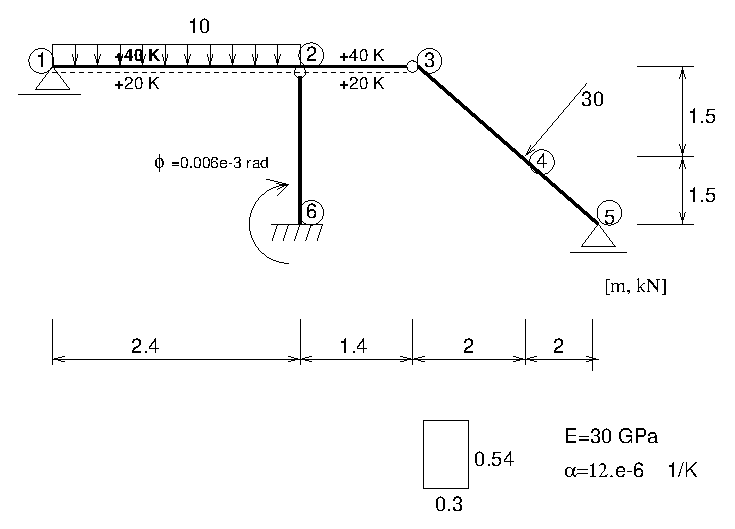
\includegraphics[width=0.7\textwidth]{ex01.eps}}
\end{htmlonly}
%begin{latexonly}
\ifpdf
\centerline{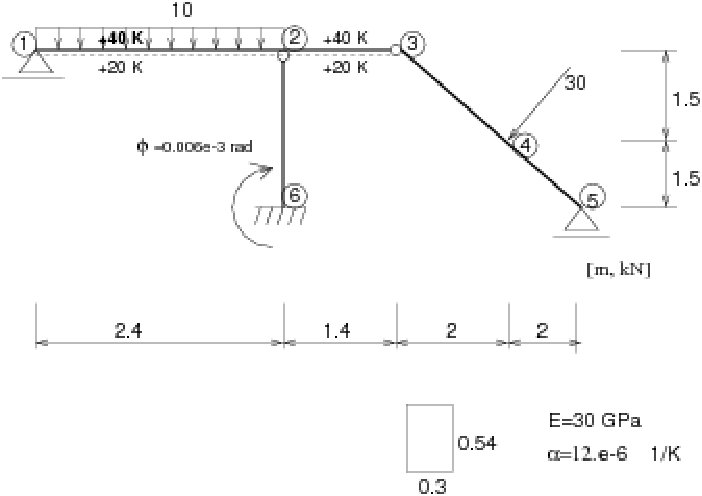
\includegraphics[width=0.7\textwidth]{ex01.pdf}}
\else
\centerline{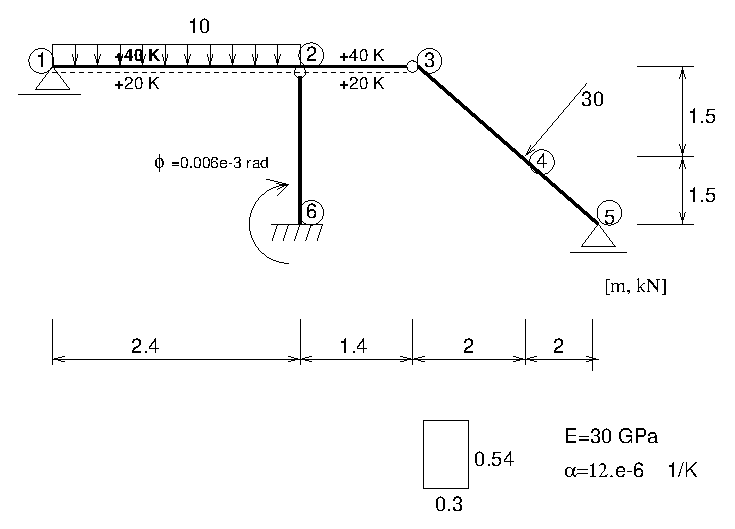
\includegraphics[width=0.7\textwidth]{ex01.eps}}
\fi
%end{latexonly}
\caption{Example 1}
\label{ex01}

\end{figure}
{\small\begin{verbatim}
test41.out
Simple Beam Structure - linear analysis
#only momentum influence to the displacements is taken into account
#beamShearCoeff is artificially enlarged.
LinearStatic 1 nsteps 3
domain 2dBeam
OutputManager tstep_all dofman_all element_all
ndofman 6 nelem 5 ncrosssect 1 nmat 1 nbc 5 nic 0 nltf 3
node 1 coords 3 0.  0.  0.  bc 3 0 1 0
node 2 coords 3 2.4 0.  0.  bc 3 0 0 0
node 3 coords 3 3.8 0.  0.  bc 3 0 0 1
node 4 coords 3 5.8 0.  1.5 bc 3 0 0 0 load 1 4
node 5 coords 3 7.8 0.  3.0 bc 3 0 1 0
node 6 coords 3 2.4 0.  3.0 bc 3 1 1 2
Beam2d 1 nodes 2 1 2 mat 1 crossSect 1 boundaryLoads  2 3 1 bodyLoads 1 5
Beam2d 2 nodes 2 2 3 mat 1 crossSect 1 DofsToCondense 1 6   bodyLoads 1 5
Beam2d 3 nodes 2 3 4 mat 1 crossSect 1 DofsToCondense 1 3
Beam2d 4 nodes 2 4 5 mat 1 crossSect 1
Beam2d 5 nodes 2 6 2 mat 1 crossSect 1 DofsToCondense 1 6
SimpleCS 1 area 0.162 Iy 0.0039366 beamShearCoeff 1.e18 thick 0.54
IsoLE 1 d 1. E 30.e6 n 0.2 tAlpha 1.2e-5
BoundaryCondition  1 loadTimeFunction 1 prescribedvalue 0.0
BoundaryCondition  2 loadTimeFunction 2 prescribedvalue -0.006e-3
ConstantEdgeLoad 3 loadTimeFunction 1 Components 3 0. 10. 0.0\
                   loadType 3 ndofs 3
NodalLoad 4 loadTimeFunction 1 Components 3 -18.0 24.0 0.0
StructTemperatureLoad 5 loadTimeFunction 3 Components 2 30.0 -20.0
PeakFunction 1 t 1.0 f(t) 1.
PeakFunction 2 t 2.0 f(t) 1.
PeakFunction 3 t 3.0 f(t) 1.
\end{verbatim}}
\subsection {Plane stress example}
\begin{figure}[tb]
\begin{htmlonly}
  \centerline{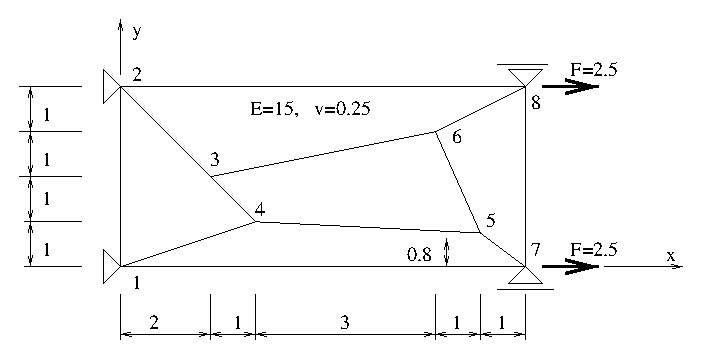
\includegraphics[width=0.7\textwidth]{ex02.eps}}
\end{htmlonly}
%begin{latexonly}
\ifpdf
\centerline{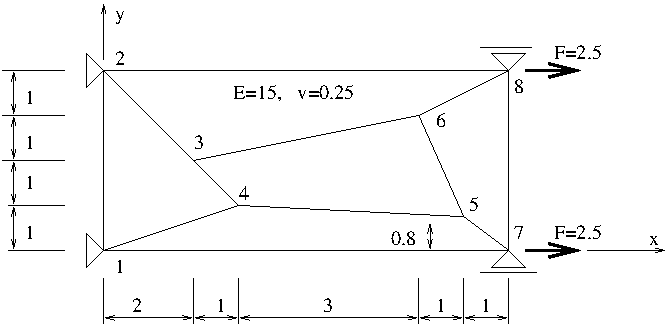
\includegraphics[width=0.7\textwidth]{ex02.pdf}}
\else
\centerline{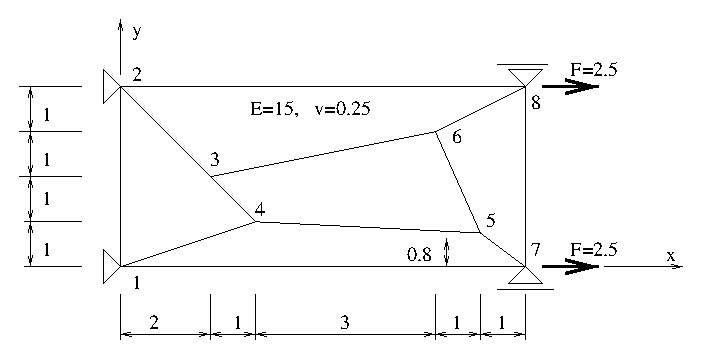
\includegraphics[width=0.7\textwidth]{ex02.eps}}
\fi
%end{latexonly}
\caption{Example 2}
\label{ex02}
\end{figure}
{\small\begin{verbatim}
patch100.out
Patch test of PlaneStress2d elements -> pure compression
LinearStatic nsteps 1
domain 2dPlaneStress
OutputManager tstep_all dofman_all element_all
ndofman 8 nelem 5 ncrosssect 1 nmat 1 nbc 2 nic 0 nltf 1
node 1 coords 3  0.0   0.0   0.0  bc 2 1 1
node 2 coords 3  0.0   4.0   0.0  bc 2 1 1
node 3 coords 3  2.0   2.0   0.0  bc 2 0 0
node 4 coords 3  3.0   1.0   0.0  bc 2 0 0
node 5 coords 3  8.0   0.8   0.0  bc 2 0 0
node 6 coords 3  7.0   3.0   0.0  bc 2 0 0
node 7 coords 3  9.0   0.0   0.0  bc 2 0 1  load 1 2
node 8 coords 3  9.0   4.0   0.0  bc 2 0 1  load 1 2
PlaneStress2d 1 nodes 4 1 4 3 2  crossSect 1 mat 1 NIP 1
PlaneStress2d 2 nodes 4 1 7 5 4  crossSect 1 mat 1 NIP 1
PlaneStress2d 3 nodes 4 4 5 6 3  crossSect 1 mat 1 NIP 1
PlaneStress2d 4 nodes 4 3 6 8 2  crossSect 1 mat 1 NIP 1
PlaneStress2d 5 nodes 4 5 7 8 6  crossSect 1 mat 1 NIP 1
SimpleCS 1 thick 1.0 width 1.0
IsoLE 1 d 0. E 15.0 n 0.25 talpha 1.0
BoundaryCondition  1 loadTimeFunction 1 prescribedvalue 0.0
NodalLoad 2 loadTimeFunction 1 Components 2 2.5 0.0
ConstantFunction 1 f(t) 1.0
\end{verbatim}}
%\vspace*{1.5cm}
%\begin{flushright}
%	 Printed on \today
%\end{flushright}


%\vfill
\section{Examples - parallel mode}
\subsection{Node-cut example}
The example shows explicit direct integration analysis of
simple structure with two DOFs.
The geometry and partitioning is sketched in
fig. \ref{nodecut-ex01}.

\begin{figure}[htb]
\begin{htmlonly}
  \centerline{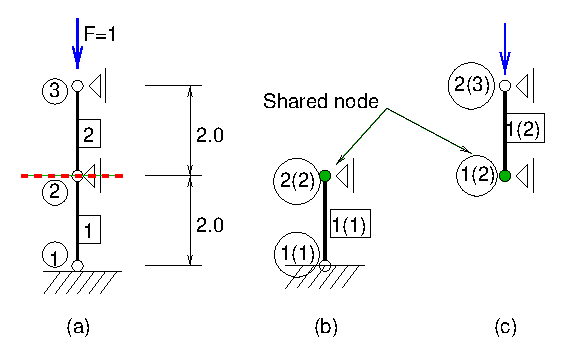
\includegraphics[width=0.7\textwidth]{poofem_ex01.eps}}
\end{htmlonly}
%begin{latexonly}
\ifpdf
\centerline{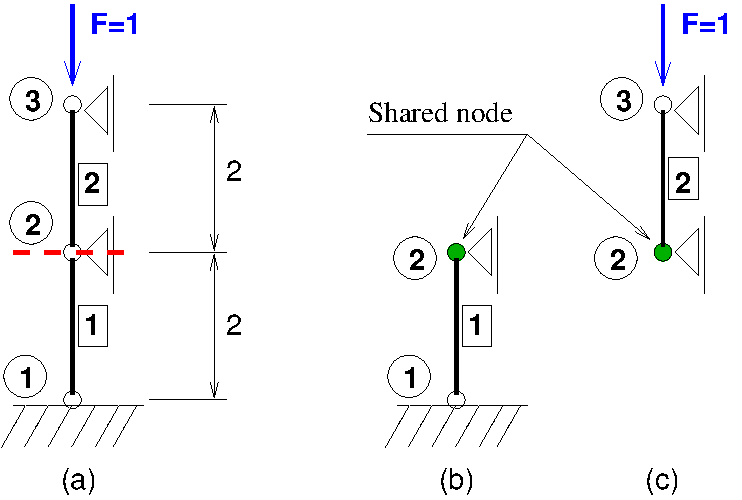
\includegraphics[width=0.7\textwidth]{poofem_ex01.pdf}}
\else
\centerline{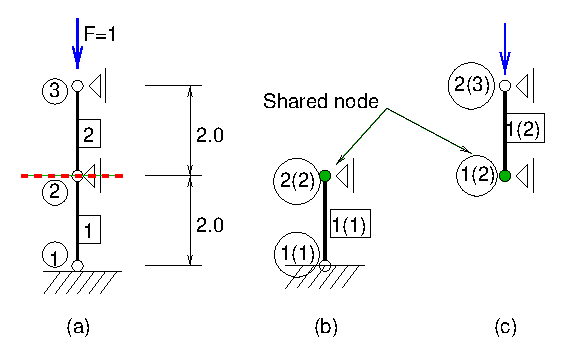
\includegraphics[width=0.7\textwidth]{poofem_ex01.eps}}
\fi
%end{latexonly}
\caption{Node-cut partitioning example: (a) whole geometry,
(b) partition~0, (c) partition~1.}
\label{nodecut-ex01}
\end{figure}

\begin{verbatim}
#
# partition 0
#
partest.out.0
Parallel test of explicit oofem computation
#
PNlDEIDynamic nsteps 3 dumpcoef 0.0 deltaT 1.0 NodeCutMode
domain 2dTruss
#
OutputManager tstep_all dofman_all element_all
ndofman 2 nelem 1 ncrosssect 1 nmat 1 nbc 2 nic 0 nltf 1
#
Node 1 coords 3 0. 0. 0. bc 2 1 1
Node 2 coords 3 0. 0. 2. bc 2 1 0 Shared partitions 1 1
Truss2d 1 nodes 2 1 2 mat 1 crossSect 1
SimpleCS 1 thick 0.1 width 10.0
IsoLE 1  tAlpha 0.000012  d 10.0  E 1.0  n 0.2
BoundaryCondition  1 loadTimeFunction 1 conditions 1 d 0.0
NodalLoad 2 loadTimeFunction 1 Components 2 0. 1.0
ConstantFunction 1 f(t) 1.0

#
# partition 1
#
partest.out.1
Parallel test of explicit oofem computation
#
PNlDEIDynamic nsteps 3 dumpcoef 0.0 deltaT 1.0 NodeCutMode
domain 2dTruss
#
OutputManager tstep_all dofman_all element_all
ndofman 2 nelem 1 ncrosssect 1 nmat 1 nbc 2 nic 0 nltf 1
#
Node 2 coords 3 0. 0. 2. bc 2 1 0 Shared partitions 1 0
Node 3 coords 3 0. 0. 4. bc 2 1 0 load 1 2
Truss2d 2 nodes 2 2 3 mat 1 crossSect 1
SimpleCS 1 thick 0.1 width 10.0
IsoLE 1  tAlpha 0.000012  d 10.0  E 1.0  n 0.2
BoundaryCondition  1 loadTimeFunction 1 conditions 1 d 0.0
NodalLoad 2 loadTimeFunction 1 Components 2 0. 1.0
ConstantFunction 1 f(t) 1.0
\end{verbatim}

\subsection{Element-cut example}
The example shows explicit direct integration analysis of
simple structure with two DOFs. The geometry and partitioning is sketched in
fig. \ref{nodecut-ex01}.

\begin{figure}[htb]
\begin{htmlonly}
  \centerline{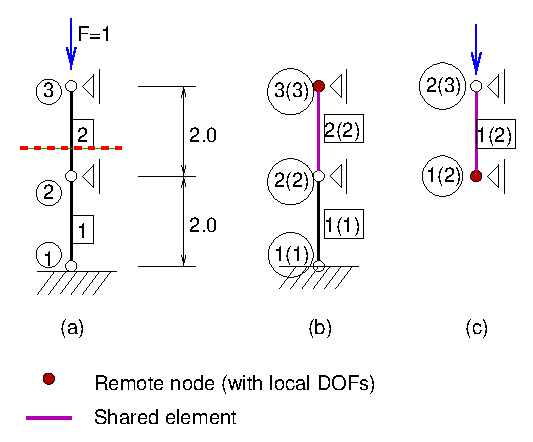
\includegraphics[width=0.7\textwidth]{poofem_ex02.eps}}
\end{htmlonly}
%begin{latexonly}
\ifpdf
\centerline{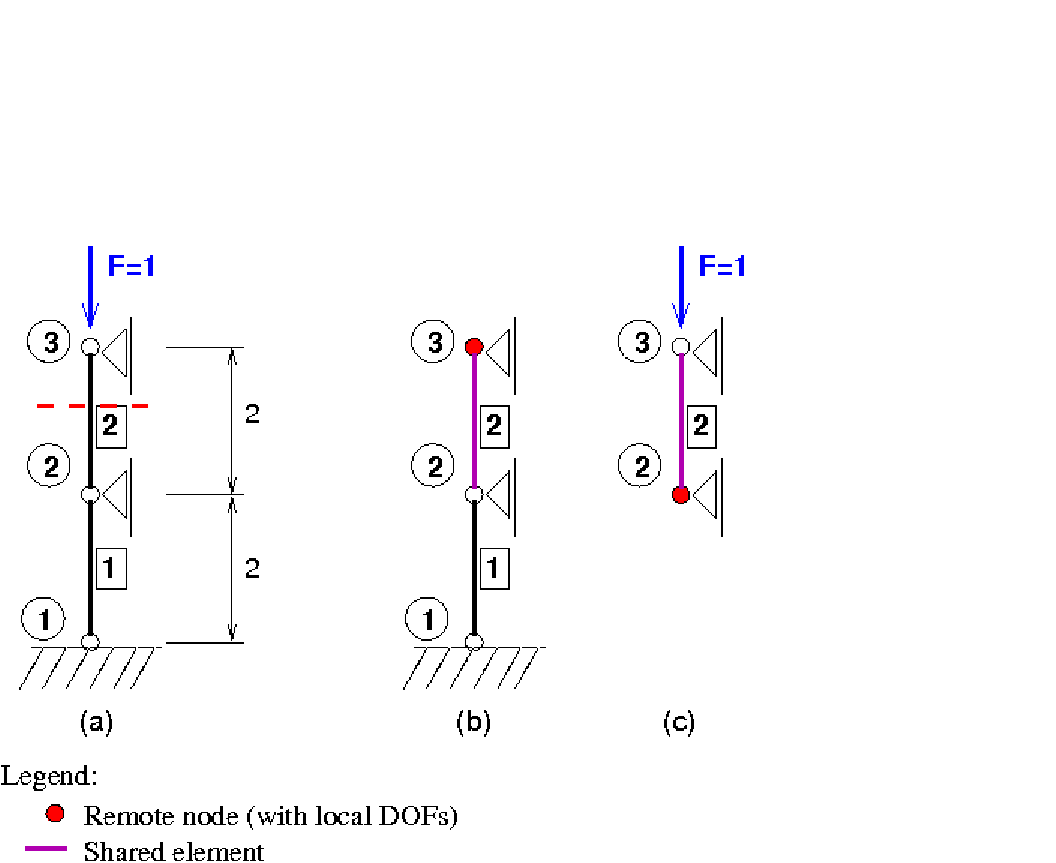
\includegraphics[width=0.7\textwidth]{poofem_ex02.pdf}}
\else
\centerline{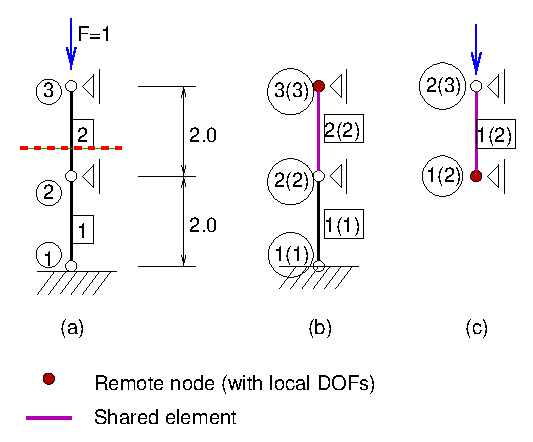
\includegraphics[width=0.7\textwidth]{poofem_ex02.eps}}
\fi
%end{latexonly}
\caption{Element-cut partitioning example: (a) whole geometry,
(b) partition~0, (c) partition~1.}
\label{elmentcut-ex02}
\end{figure}

\begin{verbatim}
#
# partition 0
#
partest2.out.0
Parallel test of explicit oofem computation
#
PNlDEIDynamic nsteps 5 dumpcoef 0.0 deltaT 1.0 ElementCutMode
domain 2dTruss
#
OutputManager tstep_all dofman_all element_all
ndofman 3 nelem 2 ncrosssect 1 nmat 1 nbc 2 nic 0 nltf 1
#
Node 1 coords 3 0. 0. 0. bc 2 1 1
Node 2 coords 3 0. 0. 2. bc 2 1 0
Node 3 coords 3 0. 0. 4. bc 2 1 0 \
       Remote partitions 1 1 load 1 2
Truss2d 1 nodes 2 1 2 mat 1 crossSect 1
Truss2d 2 nodes 2 2 3 mat 1 crossSect 1
SimpleCS 1 thick 0.1 width 10.0
IsoLE 1  tAlpha 0.000012  d 10.0  E 1.0  n 0.2
BoundaryCondition  1 loadTimeFunction 1 conditions 1 d 0.0
NodalLoad 2 loadTimeFunction 1 Components 2 0. 1.0
ConstantFunction 1 f(t) 1.0


#
# partition 1
#
partest2.out.1
Parallel test of explicit oofem computation
#
PNlDEIDynamic nsteps 5 dumpcoef 0.0 deltaT 1.0 ElementCutMode
domain 2dTruss
#
OutputManager tstep_all dofman_all element_all
ndofman 2 nelem 1 ncrosssect 1 nmat 1 nbc 2 nic 0 nltf 1
#
Node 2 coords 3 0. 0. 2. bc 2 1 0 Remote partitions 1 0
Node 3 coords 3 0. 0. 4. bc 2 1 0 load 1 2
Truss2d 2 nodes 2 2 3 mat 1 crossSect 1
SimpleCS 1 thick 0.1 width 10.0
IsoLE 1  tAlpha 0.000012  d 10.0  E 1.0  n 0.2
BoundaryCondition  1 loadTimeFunction 1 conditions 1 d 0.0
NodalLoad 2 loadTimeFunction 1 Components 2 0. 1.0
ConstantFunction 1 f(t) 1.0
\end{verbatim}

\section{Figures}
%\subsection {Node cut mode}

\begin{figure}[htb]
\begin{htmlonly}
  \centerline{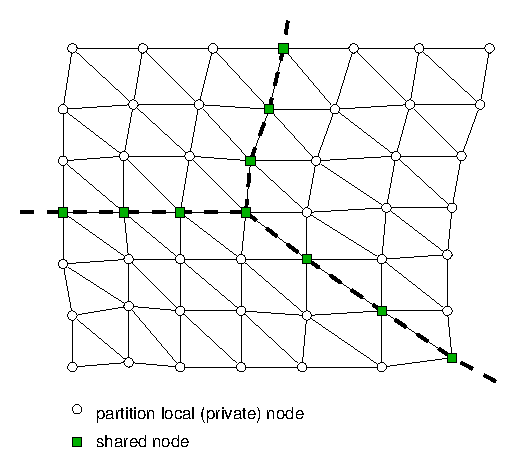
\includegraphics[width=0.7\textwidth]{nodecut0cb.eps}}
\end{htmlonly}
%begin{latexonly}
\ifpdf
\centerline{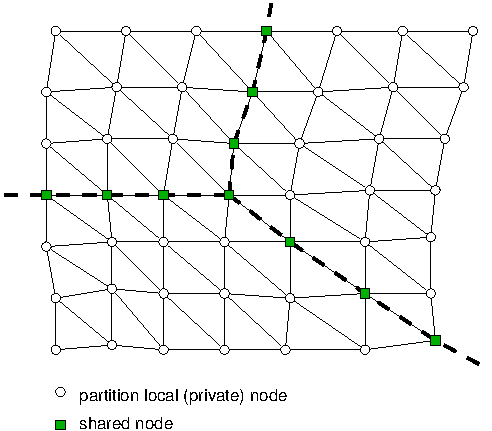
\includegraphics[width=0.7\textwidth]{nodecut0cb.pdf}}
\else
\centerline{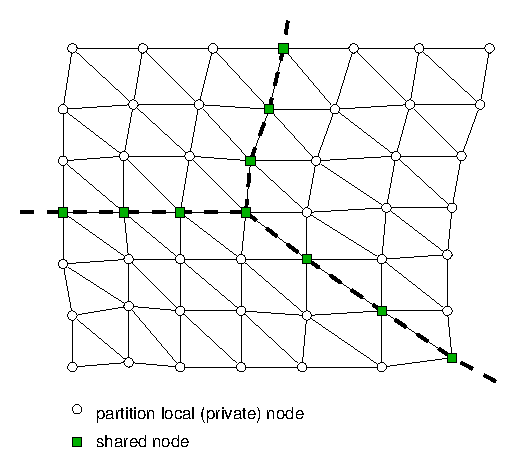
\includegraphics[width=0.7\textwidth]{nodecut0cb.eps}}
\fi
%end{latexonly}
\caption{Node-cut partitioning.}
\label{nodecut}
\end{figure}

\begin{figure}[htb]
\begin{htmlonly}
  \centerline{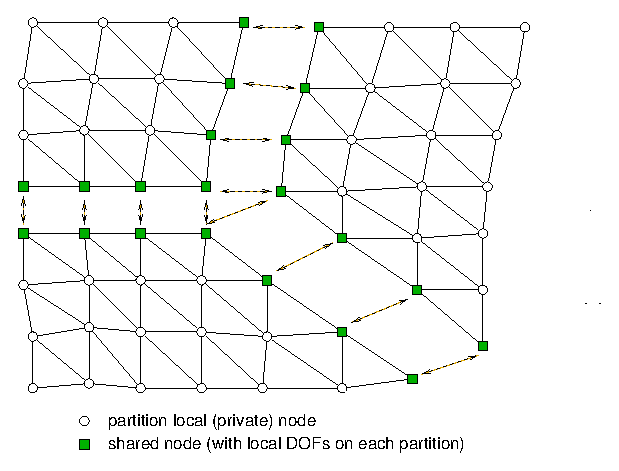
\includegraphics[width=0.7\textwidth]{nodecut1cb.eps}}
\end{htmlonly}
%begin{latexonly}
\ifpdf
\centerline{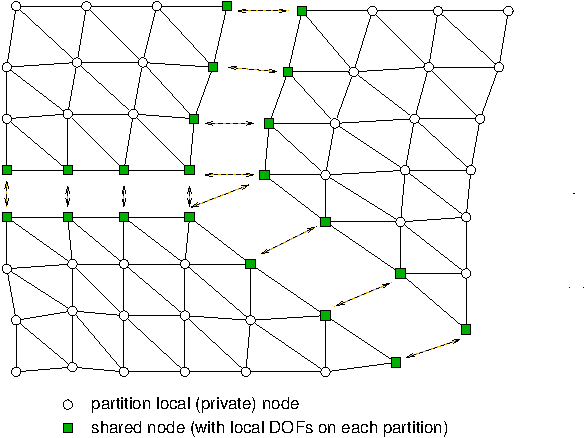
\includegraphics[width=0.7\textwidth]{nodecut1cb.pdf}}
\else
\centerline{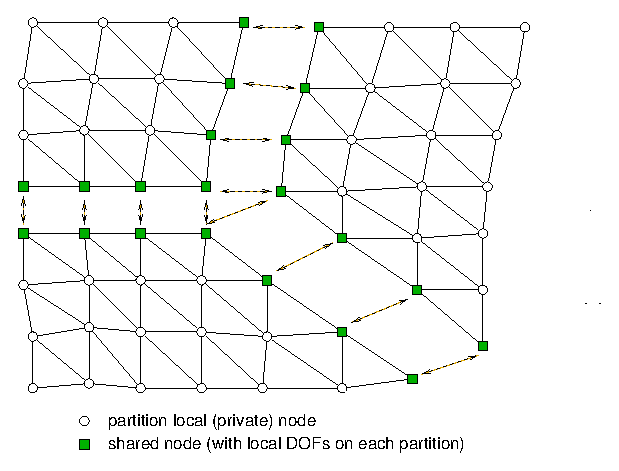
\includegraphics[width=0.7\textwidth]{nodecut1cb.eps}}
\fi
%end{latexonly}
\caption{Node-cut partitioning - local constitutive mode.}
\label{nodecut-lm}
\end{figure}

\begin{figure}[htb]
\begin{htmlonly}
  \centerline{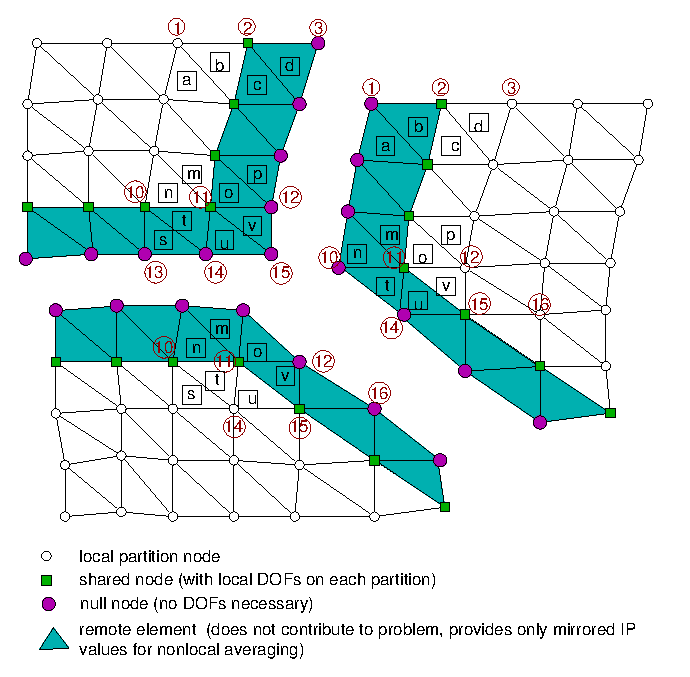
\includegraphics[width=0.7\textwidth]{nodecutnonloc1.eps}}
\end{htmlonly}
%begin{latexonly}
\ifpdf
\centerline{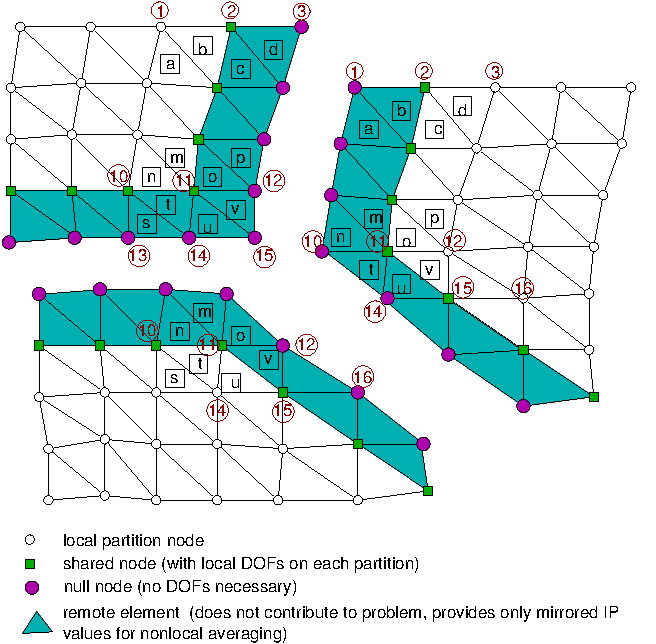
\includegraphics[width=0.7\textwidth]{nodecutnonloc1.pdf}}
\else
\centerline{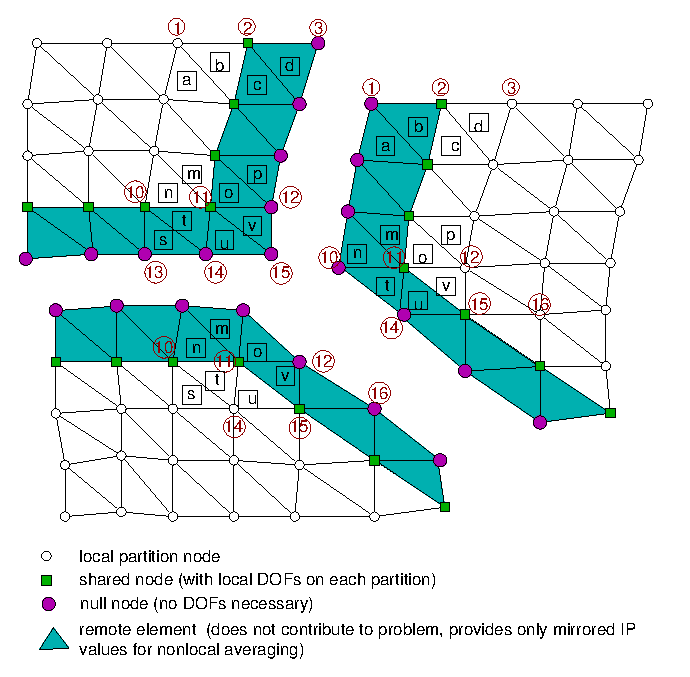
\includegraphics[width=0.7\textwidth]{nodecutnonloc1.eps}}
\fi
%end{latexonly}
\caption{Node-cut partitioning - nonlocal constitutive mode.}
\label{nodecut-nlm}
\end{figure}

%\subsection {Element cut mode}

\begin{figure}[htb]
\begin{htmlonly}
  \centerline{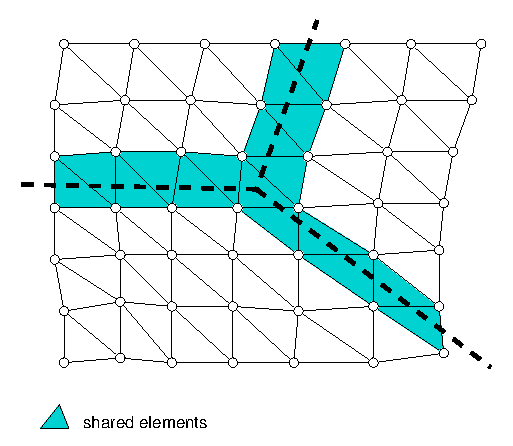
\includegraphics[width=0.7\textwidth]{elementcut0.eps}}
\end{htmlonly}
%begin{latexonly}
\ifpdf
\centerline{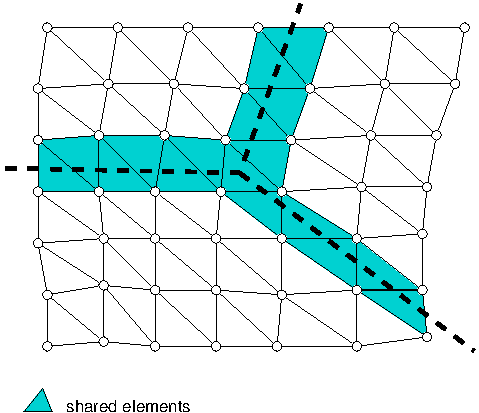
\includegraphics[width=0.7\textwidth]{elementcut0.pdf}}
\else
\centerline{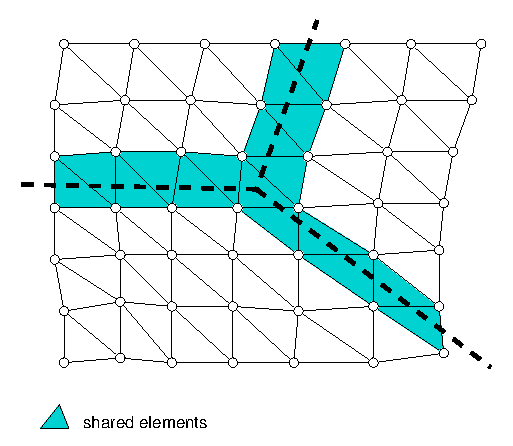
\includegraphics[width=0.7\textwidth]{elementcut0.eps}}
\fi
%end{latexonly}
\caption{Element-cut partitioning.}
\label{elmentcut}
\end{figure}

\begin{figure}[htb]
\begin{htmlonly}
  \centerline{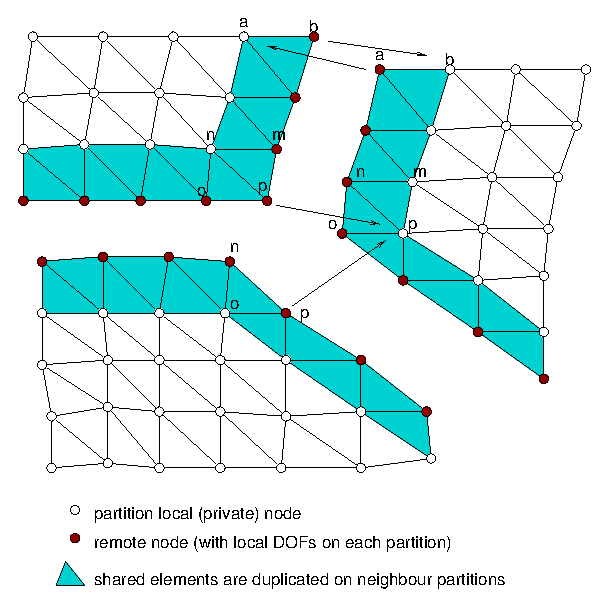
\includegraphics[width=0.7\textwidth]{elementcut1.eps}}
\end{htmlonly}
%begin{latexonly}
\ifpdf
\centerline{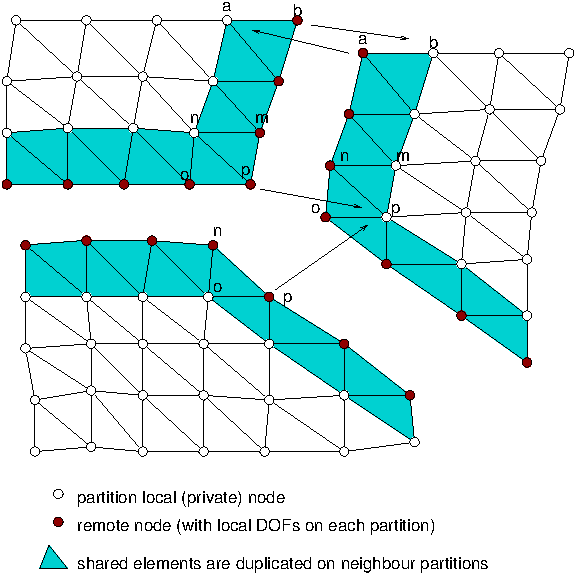
\includegraphics[width=0.7\textwidth]{elementcut1.pdf}}
\else
\centerline{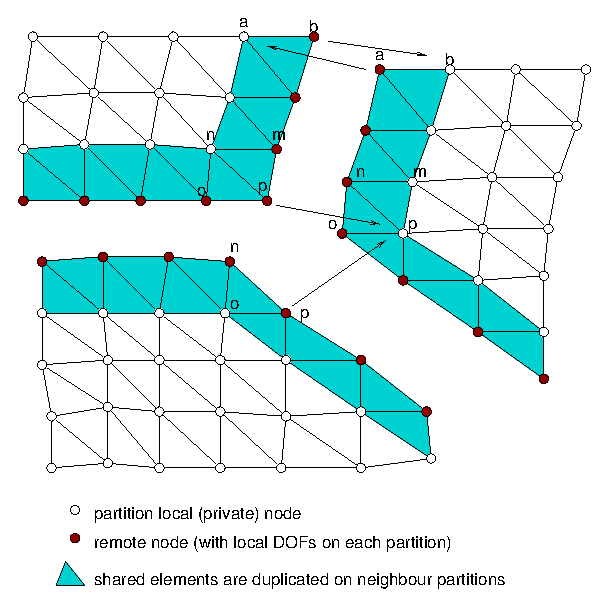
\includegraphics[width=0.7\textwidth]{elementcut1.eps}}
\fi
%end{latexonly}
\caption{Element-cut partitioning, local constitutive mode.}
\label{elmentcut-lm}
\end{figure}

\end{document}



